% --------------------------------------------------------------------------------
% ---------------------------------  Preamble  -----------------------------------
% --------------------------------------------------------------------------------

\documentclass{article}

\usepackage[nopatch=footnote]{microtype}

\hyphenpenalty=5000 \tolerance=2000 \emergencystretch=10pt

\usepackage[defaultfam,tabular]{montserrat}
\usepackage[letterpaper, margin=0.75in]{geometry}
\usepackage{graphicx}               % to insert figures
\usepackage[table,x11names]{xcolor} % colors for e-copies
\usepackage{subcaption}             % subfigures
\usepackage{placeins}               % Float barriers
\usepackage{booktabs}
\usepackage{array}
\usepackage{caption}
\usepackage{rotating}
\usepackage{multicol}
\usepackage{multirow}
\usepackage{titlesec}
\usepackage{hyperref}               % PDF hyperreferences
\usepackage{titling}
\usepackage{tikz}
\usetikzlibrary{shapes.geometric}
\usetikzlibrary{calc}
\usepackage[T1]{fontenc}
\usepackage{ifthen}
\usepackage{fancyhdr}
\usepackage{setspace}
\usepackage{eqparbox}
\renewcommand*\oldstylenums[1]{{\fontfamily{Montserrat-TOsF}\selectfont #1}}
\usepackage{enumitem}
\setlist[itemize]{topsep=0pt}
\setlist[enumerate]{topsep=0pt}

\makeatletter
\renewcommand{\@dotsep}{10000} 
\makeatother

\newsavebox{\savefig}

\newcommand{\Vline}[1]{\vrule width #1}
\newcommand{\Hline}[1]{\noalign{\hrule height #1}}

\setcounter{secnumdepth}{0}

\titleformat{\section}[block]
  {\normalfont\fontsize{16}{17}\fontseries{ub}\selectfont}
  {\thesection\enspace}{0pt}{\centering\MakeUppercase}[\vspace{2pt}{\titlerule[2pt]}]

\titleformat{\subsection}[block]
  {{\titlerule[1pt]}\addvspace{3pt}\bfseries\centering}
  {\thesection\enspace}{0pt}{\MakeUppercase}[\vspace{3pt}{\titlerule[1pt]}]

\titleformat{\subsubsection} [block]{\bfseries}{}{0em}{\MakeUppercase}

\renewcommand\maketitlehooka{\null\mbox{}\vfill}
\renewcommand\maketitlehookd{\vfill\null}
\title{
  \fontfamily{Montserrat-TOsF}\selectfont
  \vspace{6px}
  \fontsize{50}{60}\fontseries{ub}\selectfont\textcolor{white}{\MakeUppercase{B}}\fontsize{45}{55}\fontseries{ub}\selectfont\textcolor{white}{\MakeUppercase{attle}}\fontsize{50}{60}\fontseries{ub}\selectfont\textcolor{white}{\MakeUppercase{T}}\fontsize{45}{55}\fontseries{ub}\selectfont\textcolor{white}{\MakeUppercase{ech}}\\
  \fontsize{35}{42}\fontseries{ub}\selectfont\MakeUppercase{Outworlds Wastes}\\
  ~\\
  \href{https://ko-fi.com/bleptarts}{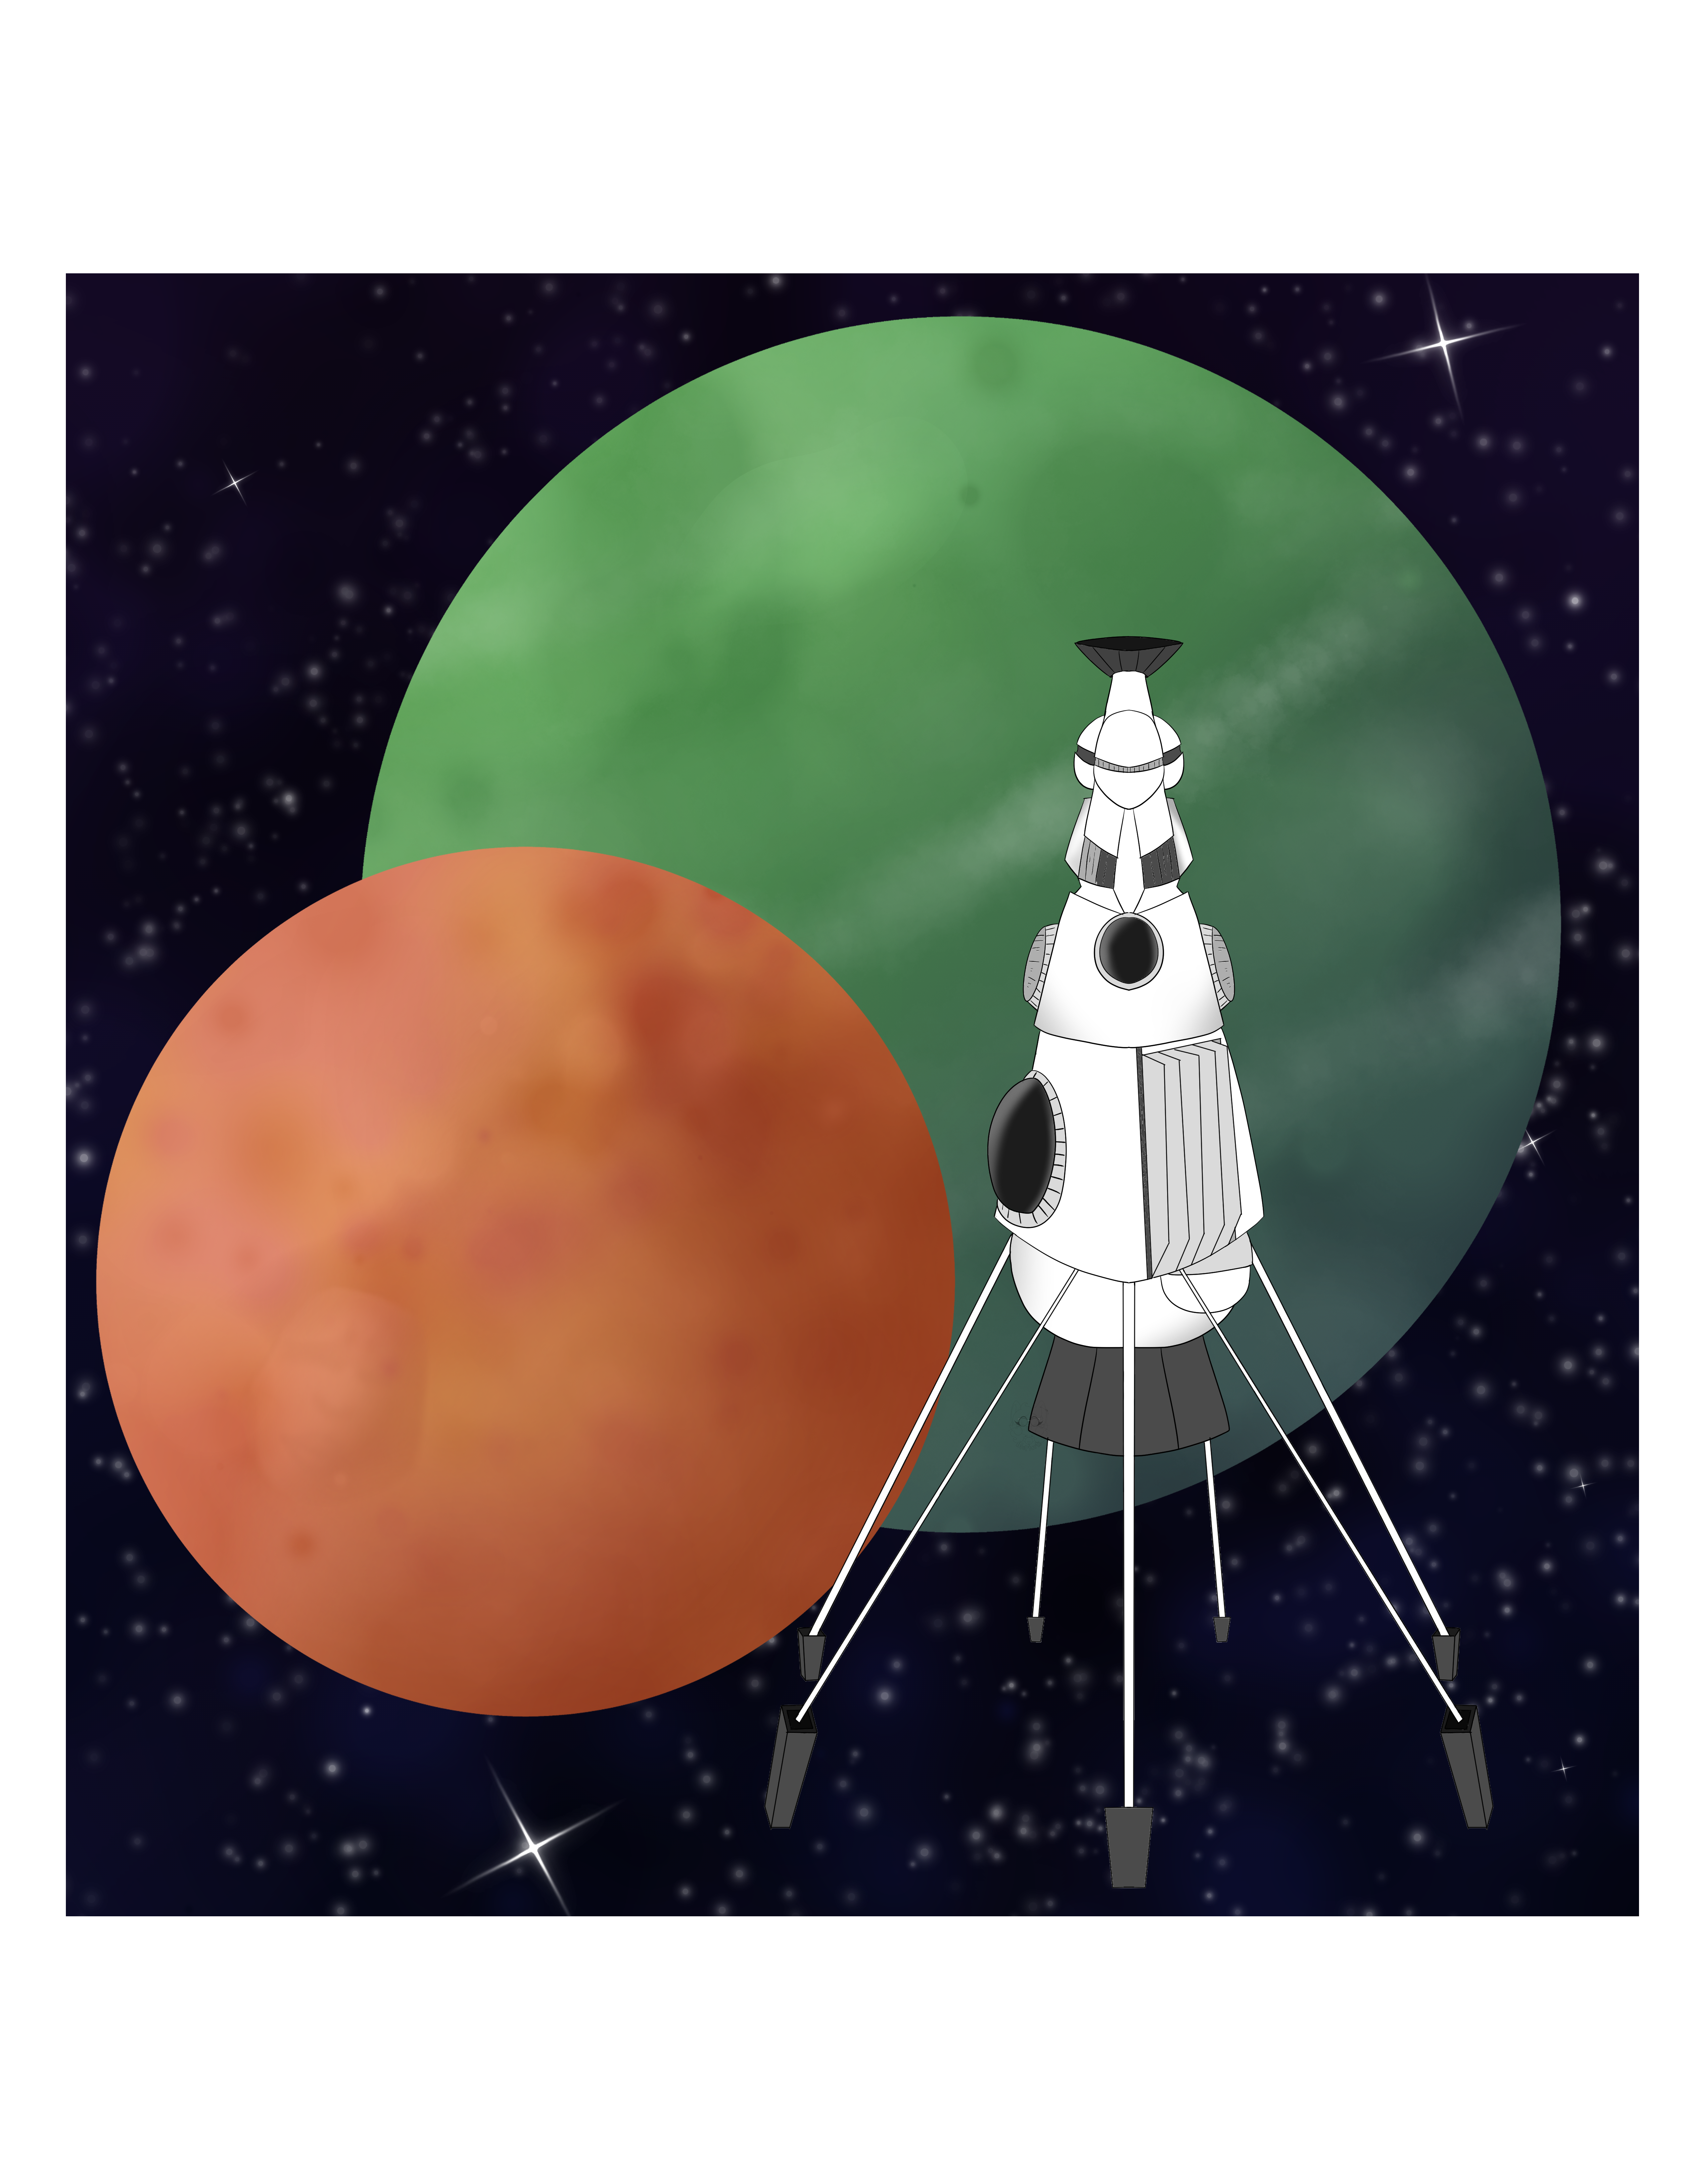
\includegraphics[alt='Outworlds Wastes logo', height=4in]{img/Outworlds-Wastes.png}}
  ~\\
  ~\\
  \LARGE\bfseries{Lightweight Narrative League Framework} \\
}
\author{}
\date{}

% Optional PDF information
\ifpdf
\hypersetup{
  pdftitle={Outworlds Wastes},
  pdfauthor={Jeremy L Thompson},
  pdfsubject={BattleTech},
  pdfkeywords={BattleTech}
}
\fi

\setlength\parskip{5pt plus 2pt minus 1pt}

\newcommand{\outworldsMode}{mode-pdf}

\definecolor{background-green}{RGB}{49, 56, 49}
\definecolor{background-tan}{RGB}{204, 197, 179}
\definecolor{background-gray}{RGB}{255, 252, 247}

% --------------------------------------------------------------------------------
% ---------------------------------  Document  -----------------------------------
% --------------------------------------------------------------------------------

\begin{document}

\pagestyle{fancy}
\fancyhead{}
\renewcommand{\headrulewidth}{2pt}% default is 0pt
\fancyfoot{}
\renewcommand{\footrulewidth}{1pt}% default is 0pt
\fancyfoot[C]{\eqmakebox[text][r]{BattleTech} \hspace{0.1em} \eqmakebox[num][c]{\bfseries\LARGE \raisebox{-.2ex}{\thepage}} \hspace{0.1em} \eqmakebox[text][l]{Outworlds Wastes}}

\clearpage

% --------------------------------------------------------------------------------
\maketitle
% --------------------------------------------------------------------------------

\AddToHookNext{shipout/background}
{\put(0,-\paperheight)
  {%
   
\begin{tikzpicture}
   \fill[use as bounding box,background-tan] (current page.north west) rectangle (\paperwidth,0);
   \fill[use as bounding box,background-green] ($ (current page.north west)+(0,-5.35) $) rectangle ++(\paperwidth,-1.7);
   \fill[use as bounding box,background-gray] ($ (current page.north west)+(0,-7.05) $) rectangle ++(\paperwidth,-1.6);
   \fill[use as bounding box,background-gray] ($ (current page.north west)+(0,-21.5) $) rectangle ++(\paperwidth,-0.9);
   \end{tikzpicture}
  }
}

\thispagestyle{empty}

\pagenumbering{roman}
\newpage
\pagenumbering{arabic}

\setlength{\headsep}{10pt}

% --------------------------------------------------------------------------------
\section{BattleTech: Outworlds Wastes}
% --------------------------------------------------------------------------------

The event format provides faster, simplified rules which are more suitable for playing multiple scenarios in a large event, such as at a convention.


% --------------------------------------------------------------------------------
\subsection{Force Construction}
\label{subsec:force_construction}
% --------------------------------------------------------------------------------

Commanders create an initial force of up to 10,000 BV.
BV costs for all units are listed in the \href{http://www.masterunitlist.info}{Master Unit List} or \href{https://megamek.org}{MegaMekLab}.
Force construction must follow the following rules:

\begin{itemize}

\item Commanders have a modified Union class DropShip with 15 configurable bays.
Bays may be empty and can changed to a different configuration.
Bay space for all infantry units is shared across bays.
Your entire force must fit onto your DropShip.
Bay limits are in the table below.

\begin{table}[!h]
\ifthenelse{\not \equal{\outworldsMode}{mode-web}}{\fontfamily{Montserrat-LF}}{\small}\selectfont
\centering
\newcolumntype{R}[1]{>{\raggedleft\let\newline\\\arraybackslash\hspace{0pt}}m{#1}}
\begin{tabular}{!{\Vline{1pt}} m{10em} m{20em} R{3.8em} !{\Vline{1pt}}}
\Hline{1pt}
\rowcolor{black!30}  \bfseries{Bay Type} & \bfseries{Capacity} & \bfseries{Limit} \\
\Hline{1pt}
'Mech            & 1 'Mech or 1/2 superheavy 'Mech    & 12 bays \\
Combat Vehicle   & 2 vehicles or 1 superheavy vehicle & 5 bays  \\
Aerospace        & 1 aerospace unit                   & 2 bays  \\
ProtoMech        & 5 ProtoMechs                       & 2 bays  \\
Infantry         & 15 tons or 1 unit over 15 tons     & 2 bays  \\
\Hline{1pt}
\end{tabular}
\caption*{DropShip Bay Limits}
\end{table}

Support, Advanced Support, and Advanced Aerospace units are not permitted.
Illegal designs and units over 200 tons are also not permitted.
Units over 100 tons, such as superheavy 'Mechs, require double the bay space as standard units.

\item Commanders must select units from their faction on the \href{http://www.masterunitlist.info/}{Master Unit List} for the era chosen by league organizers.
Forces can include units with introductory, standard, or advanced technology.
For example, the Marauder MAD-3R is a valid ilClan era mercenary unit.

\item Forces may include one Unique or Experimental unit.
The Unique unit may be Extinct if another variant of the unit is available to the faction in the current era and the faction has the relevant technology base to recreate the unit.

\item Each force can start with no more than 7,000 BV in 'Mechs.
Commanders are encouraged to try to use the typical 'Mech unit composition of their faction.

\item Some scenarios will require infantry/Battle Armor or Combat Vehicles with cargo capacity, so commanders should have at least one of each of these units in their force.

\item Unless optional Battlefield Support or off-board artillery rules are used, a force can only include on-map units.
For example, artillery and aerospace units can only be used on-map by default.

\item The BV cost of a unit includes the skill level.
The initial skill levels for a unit may be no better than Gunnery 3/Piloting 4 and cannot differ by more than 3.
Average skill levels for factions and units are given on \emph{BattleTech: Total Warfare} p. 40.
ProtoMechs always have Piloting 5 and infantry units without anti-'Mech equipment have Anti-'Mech 5, because these skills are not used for these units.

\end{itemize}

Commanders are responsible for knowing which rulebooks contain the rules pertaining to all units and special equipment in their force.

Unit record sheets can be generated using \href{https://megamek.org}{MegaMekLab} or similar tools.
BV costs sometimes do not mach between the \href{http://www.masterunitlist.info}{Master Unit List} and \href{https://megamek.org}{MegaMekLab}, especially for infantry units.
Commanders must use the same source for all BV costs.
All record sheets must agree with the BV costs from this source.

Learning new types of units can be intimidating.
Commanders may limit the types of different units in their non-'Mech forces.
For example, a force could include only troop transports and Battle Armor so the commander can meet any objectives while keeping new rules to a minimum.


\newpage

% --------------------------------------------------------------------------------
\subsection{Sample Forces}
\label{subsec:sample_forces}
% --------------------------------------------------------------------------------

Two sample initial forces are provided below.
The first force is a Civil War era mercenary company and the second force is an ilClan era Raven Alliance Nova.
Pilot names are encouraged, as one of the goals of \emph{BattleTech: Outworlds Wastes} is to develop the personalized lore for your force.

\begin{table}[!h]
\ifthenelse{\not \equal{\outworldsMode}{mode-web}}{\fontfamily{Montserrat-LF}}{\small}\selectfont
\centering
\newcolumntype{R}[1]{>{\raggedleft\let\newline\\\arraybackslash\hspace{0pt}}m{#1}}
\begin{tabular}{!{\Vline{1pt}} m{2em} m{12em} m{8em} R{4.6em} R{4.6em} R{3.5em} R{3.8em} !{\Vline{1pt}}}
\Hline{1pt}
\rowcolor{black!30}  \bfseries{Bay} & \bfseries{Unit} & \bfseries{Pilot} & \bfseries{Gunnery} & \bfseries{Piloting} & \bfseries{BV} & \bfseries{Adj BV} \\
\Hline{1pt}
\rowcolor{black!30} \multicolumn{7}{!{\Vline{1pt}}c!{\Vline{1pt}}}{'Mechs} \\
\Hline{1pt}
1   & Atlas AS7-D           & 'Meg' Courant    & 3       & 4         & 1,897 & 2,504 \\
2   & Phoenix Hawk PXH-2K   & 'Bison' Helge    & 4       & 5         & 1,271 & 1,271 \\
3   & Blackjack BJ-2        & 'Lizard' Baker   & 4       & 5         & 1,148 & 1,148 \\
4   & Locust IIC            & 'Casper' Poole   & 4       & 5         & 1,100 & 1,100 \\
\Hline{1pt}
\rowcolor{black!30}\multicolumn{7}{!{\Vline{1pt}}c!{\Vline{1pt}}}{Combat Vehicles} \\
\Hline{1pt}
1  & Maxim Hover Transport &                   & 4       & 5         &   764 &   764 \\
1  & Maxim Hover Transport &                   & 4       & 5         &   764 &   764 \\
2  & Galleon GAL-102       &                   & 4       & 5         &   651 &   651 \\
2  & Galleon GAL-102       &                   & 4       & 5         &   651 &   651 \\
3  & Warrior H-7           &                   & 4       & 5         &   295 &   295 \\
3  & Warrior H-7           &                   & 4       & 5         &   295 &   295 \\
\Hline{1pt}
\rowcolor{black!30}\multicolumn{7}{!{\Vline{1pt}}c!{\Vline{1pt}}}{Infantry/Battle Armor} \\
\Hline{1pt}
1  & IS Std BA, LRR        &                   & 4       & 5         &   255 &   255 \\
1  & IS Std BA, Laser      &                   & 4       & 5         &   231 &   231 \\
\Hline{1pt}
8  & Total Bays            &                   &         &           &       &       \\
   & Total BV              &                   &         &           &       & 9,929 \\
\Hline{1pt}
\end{tabular}
\caption*{Civil War Era Mercenary Force - Meg's Magpies}
\end{table}

\begin{table}[!h]
\ifthenelse{\not \equal{\outworldsMode}{mode-web}}{\fontfamily{Montserrat-LF}}{\small}\selectfont
\centering
\newcolumntype{R}[1]{>{\raggedleft\let\newline\\\arraybackslash\hspace{0pt}}m{#1}}
\begin{tabular}{!{\Vline{1pt}} m{2em} m{12em} m{8em} R{4.6em} R{4.6em} R{3.5em} R{3.8em} !{\Vline{1pt}}}
\Hline{1pt}
\rowcolor{black!30}  \bfseries{Bay} & \bfseries{Unit} & \bfseries{Pilot} & \bfseries{Gunnery} & \bfseries{Piloting} & \bfseries{BV} & \bfseries{Adj BV} \\
\Hline{1pt}
\rowcolor{black!30}\multicolumn{7}{!{\Vline{1pt}}c!{\Vline{1pt}}}{'Mechs} \\
\Hline{1pt}
1 & Carrion Crow A        & Sarah Magnus    & 3       & 4         & 1,622 & 2,141 \\
2 & Nova U                &       Bryn      & 4       & 5         & 1,413 & 1,413 \\
3 & Adder J               &       Ada       & 4       & 5         & 1,222 & 1,222 \\
4 & Kit Fox V             &       Soton     & 3       & 4         &   974 & 1,286 \\
5 & Fire Moth A           &       Tina      & 3       & 4         &   639 &   843 \\
\Hline{1pt}
\rowcolor{black!30}\multicolumn{7}{!{\Vline{1pt}}c!{\Vline{1pt}}}{Combat Vehicles} \\
\Hline{1pt}
1 & Karnov UR Transport   &                 & 4       & 5          &   125 &   125 \\
\Hline{1pt}
\rowcolor{black!30}\multicolumn{7}{!{\Vline{1pt}}c!{\Vline{1pt}}}{Infantry/Battle Armor} \\
\Hline{1pt}
1 & Elemental BA, Laser   &                 & 3       & 4         &   447 &   590 \\
1 & Elemental BA, HMG     &                 & 3       & 4         &   415 &   548 \\
1 & Elemental BA, Flamer  &                 & 3       & 4         &   404 &   533 \\
2 & Elemental BA, Flamer  &                 & 3       & 4         &   404 &   533 \\
2 & Gnome BA              &                 & 3       & 4         &   580 &   766 \\
\Hline{1pt}
8 & Total Bays            &                 &         &           &       &       \\
  & Total BV              &                 &         &           &       & 10,000 \\
\Hline{1pt}
\end{tabular}
\caption*{ilClan Era Raven Alliance Force - Raven Expeditionary Cluster, Alpha Nova}
\end{table}

Both forces can support additional units on their DropShips.
However, the Raven Alliance force cannot add any additional infantry bays because the DropShip has the maximum of 5 infantry bays.


\newpage

% --------------------------------------------------------------------------------
\subsection{Advanced Force Construction Rules}
% --------------------------------------------------------------------------------

\input{2-Force-Construction/2-Advanced-Force-Construction.tex}

\begin{figure}[!h]
  \begin{center}
  \begin{subfigure}{0.4\textwidth}
    \centering
    \frame{\includegraphics[alt='Clan Dark Caste Faction list', height=4.9in, width=2.4in]{img/Dark-Caste-List.png}}
    \caption*{Clan Dark Caste\\Civil War Era}
  \end{subfigure}
  \hspace{1in}
  \begin{subfigure}{0.4\textwidth}
    \centering
    \frame{\includegraphics[alt='Combine Mercenary Faction list', height=4.9in, width=2.4in]{img/Combine-Mercenary-List.png}}
    \caption*{Combine Mercenary\\Clan Invasion Era}
  \end{subfigure}
  \ifthenelse{\equal{\outworldsMode}{mode-pdf}}{\caption*{Custom Faction Lists}}{}
  \end{center}
\end{figure}


\newpage


\newpage

% --------------------------------------------------------------------------------
\begin{spacing}{0.1}
\tableofcontents
\end{spacing}
% --------------------------------------------------------------------------------

\newpage

% --------------------------------------------------------------------------------
\section{Background}
% --------------------------------------------------------------------------------

The event format provides faster, simplified rules which are more suitable for playing multiple scenarios in a large event, such as at a convention.


% --------------------------------------------------------------------------------
\subsection{Force Construction}
\label{subsec:force_construction}
% --------------------------------------------------------------------------------

Commanders create an initial force of up to 10,000 BV.
BV costs for all units are listed in the \href{http://www.masterunitlist.info}{Master Unit List} or \href{https://megamek.org}{MegaMekLab}.
Force construction must follow the following rules:

\begin{itemize}

\item Commanders have a modified Union class DropShip with 15 configurable bays.
Bays may be empty and can changed to a different configuration.
Bay space for all infantry units is shared across bays.
Your entire force must fit onto your DropShip.
Bay limits are in the table below.

\begin{table}[!h]
\ifthenelse{\not \equal{\outworldsMode}{mode-web}}{\fontfamily{Montserrat-LF}}{\small}\selectfont
\centering
\newcolumntype{R}[1]{>{\raggedleft\let\newline\\\arraybackslash\hspace{0pt}}m{#1}}
\begin{tabular}{!{\Vline{1pt}} m{10em} m{20em} R{3.8em} !{\Vline{1pt}}}
\Hline{1pt}
\rowcolor{black!30}  \bfseries{Bay Type} & \bfseries{Capacity} & \bfseries{Limit} \\
\Hline{1pt}
'Mech            & 1 'Mech or 1/2 superheavy 'Mech    & 12 bays \\
Combat Vehicle   & 2 vehicles or 1 superheavy vehicle & 5 bays  \\
Aerospace        & 1 aerospace unit                   & 2 bays  \\
ProtoMech        & 5 ProtoMechs                       & 2 bays  \\
Infantry         & 15 tons or 1 unit over 15 tons     & 2 bays  \\
\Hline{1pt}
\end{tabular}
\caption*{DropShip Bay Limits}
\end{table}

Support, Advanced Support, and Advanced Aerospace units are not permitted.
Illegal designs and units over 200 tons are also not permitted.
Units over 100 tons, such as superheavy 'Mechs, require double the bay space as standard units.

\item Commanders must select units from their faction on the \href{http://www.masterunitlist.info/}{Master Unit List} for the era chosen by league organizers.
Forces can include units with introductory, standard, or advanced technology.
For example, the Marauder MAD-3R is a valid ilClan era mercenary unit.

\item Forces may include one Unique or Experimental unit.
The Unique unit may be Extinct if another variant of the unit is available to the faction in the current era and the faction has the relevant technology base to recreate the unit.

\item Each force can start with no more than 7,000 BV in 'Mechs.
Commanders are encouraged to try to use the typical 'Mech unit composition of their faction.

\item Some scenarios will require infantry/Battle Armor or Combat Vehicles with cargo capacity, so commanders should have at least one of each of these units in their force.

\item Unless optional Battlefield Support or off-board artillery rules are used, a force can only include on-map units.
For example, artillery and aerospace units can only be used on-map by default.

\item The BV cost of a unit includes the skill level.
The initial skill levels for a unit may be no better than Gunnery 3/Piloting 4 and cannot differ by more than 3.
Average skill levels for factions and units are given on \emph{BattleTech: Total Warfare} p. 40.
ProtoMechs always have Piloting 5 and infantry units without anti-'Mech equipment have Anti-'Mech 5, because these skills are not used for these units.

\end{itemize}

Commanders are responsible for knowing which rulebooks contain the rules pertaining to all units and special equipment in their force.

Unit record sheets can be generated using \href{https://megamek.org}{MegaMekLab} or similar tools.
BV costs sometimes do not mach between the \href{http://www.masterunitlist.info}{Master Unit List} and \href{https://megamek.org}{MegaMekLab}, especially for infantry units.
Commanders must use the same source for all BV costs.
All record sheets must agree with the BV costs from this source.

Learning new types of units can be intimidating.
Commanders may limit the types of different units in their non-'Mech forces.
For example, a force could include only troop transports and Battle Armor so the commander can meet any objectives while keeping new rules to a minimum.


\newpage

% --------------------------------------------------------------------------------
\subsection{Sample Forces}
\label{subsec:sample_forces}
% --------------------------------------------------------------------------------

Two sample initial forces are provided below.
The first force is a Civil War era mercenary company and the second force is an ilClan era Raven Alliance Nova.
Pilot names are encouraged, as one of the goals of \emph{BattleTech: Outworlds Wastes} is to develop the personalized lore for your force.

\begin{table}[!h]
\ifthenelse{\not \equal{\outworldsMode}{mode-web}}{\fontfamily{Montserrat-LF}}{\small}\selectfont
\centering
\newcolumntype{R}[1]{>{\raggedleft\let\newline\\\arraybackslash\hspace{0pt}}m{#1}}
\begin{tabular}{!{\Vline{1pt}} m{2em} m{12em} m{8em} R{4.6em} R{4.6em} R{3.5em} R{3.8em} !{\Vline{1pt}}}
\Hline{1pt}
\rowcolor{black!30}  \bfseries{Bay} & \bfseries{Unit} & \bfseries{Pilot} & \bfseries{Gunnery} & \bfseries{Piloting} & \bfseries{BV} & \bfseries{Adj BV} \\
\Hline{1pt}
\rowcolor{black!30} \multicolumn{7}{!{\Vline{1pt}}c!{\Vline{1pt}}}{'Mechs} \\
\Hline{1pt}
1   & Atlas AS7-D           & 'Meg' Courant    & 3       & 4         & 1,897 & 2,504 \\
2   & Phoenix Hawk PXH-2K   & 'Bison' Helge    & 4       & 5         & 1,271 & 1,271 \\
3   & Blackjack BJ-2        & 'Lizard' Baker   & 4       & 5         & 1,148 & 1,148 \\
4   & Locust IIC            & 'Casper' Poole   & 4       & 5         & 1,100 & 1,100 \\
\Hline{1pt}
\rowcolor{black!30}\multicolumn{7}{!{\Vline{1pt}}c!{\Vline{1pt}}}{Combat Vehicles} \\
\Hline{1pt}
1  & Maxim Hover Transport &                   & 4       & 5         &   764 &   764 \\
1  & Maxim Hover Transport &                   & 4       & 5         &   764 &   764 \\
2  & Galleon GAL-102       &                   & 4       & 5         &   651 &   651 \\
2  & Galleon GAL-102       &                   & 4       & 5         &   651 &   651 \\
3  & Warrior H-7           &                   & 4       & 5         &   295 &   295 \\
3  & Warrior H-7           &                   & 4       & 5         &   295 &   295 \\
\Hline{1pt}
\rowcolor{black!30}\multicolumn{7}{!{\Vline{1pt}}c!{\Vline{1pt}}}{Infantry/Battle Armor} \\
\Hline{1pt}
1  & IS Std BA, LRR        &                   & 4       & 5         &   255 &   255 \\
1  & IS Std BA, Laser      &                   & 4       & 5         &   231 &   231 \\
\Hline{1pt}
8  & Total Bays            &                   &         &           &       &       \\
   & Total BV              &                   &         &           &       & 9,929 \\
\Hline{1pt}
\end{tabular}
\caption*{Civil War Era Mercenary Force - Meg's Magpies}
\end{table}

\begin{table}[!h]
\ifthenelse{\not \equal{\outworldsMode}{mode-web}}{\fontfamily{Montserrat-LF}}{\small}\selectfont
\centering
\newcolumntype{R}[1]{>{\raggedleft\let\newline\\\arraybackslash\hspace{0pt}}m{#1}}
\begin{tabular}{!{\Vline{1pt}} m{2em} m{12em} m{8em} R{4.6em} R{4.6em} R{3.5em} R{3.8em} !{\Vline{1pt}}}
\Hline{1pt}
\rowcolor{black!30}  \bfseries{Bay} & \bfseries{Unit} & \bfseries{Pilot} & \bfseries{Gunnery} & \bfseries{Piloting} & \bfseries{BV} & \bfseries{Adj BV} \\
\Hline{1pt}
\rowcolor{black!30}\multicolumn{7}{!{\Vline{1pt}}c!{\Vline{1pt}}}{'Mechs} \\
\Hline{1pt}
1 & Carrion Crow A        & Sarah Magnus    & 3       & 4         & 1,622 & 2,141 \\
2 & Nova U                &       Bryn      & 4       & 5         & 1,413 & 1,413 \\
3 & Adder J               &       Ada       & 4       & 5         & 1,222 & 1,222 \\
4 & Kit Fox V             &       Soton     & 3       & 4         &   974 & 1,286 \\
5 & Fire Moth A           &       Tina      & 3       & 4         &   639 &   843 \\
\Hline{1pt}
\rowcolor{black!30}\multicolumn{7}{!{\Vline{1pt}}c!{\Vline{1pt}}}{Combat Vehicles} \\
\Hline{1pt}
1 & Karnov UR Transport   &                 & 4       & 5          &   125 &   125 \\
\Hline{1pt}
\rowcolor{black!30}\multicolumn{7}{!{\Vline{1pt}}c!{\Vline{1pt}}}{Infantry/Battle Armor} \\
\Hline{1pt}
1 & Elemental BA, Laser   &                 & 3       & 4         &   447 &   590 \\
1 & Elemental BA, HMG     &                 & 3       & 4         &   415 &   548 \\
1 & Elemental BA, Flamer  &                 & 3       & 4         &   404 &   533 \\
2 & Elemental BA, Flamer  &                 & 3       & 4         &   404 &   533 \\
2 & Gnome BA              &                 & 3       & 4         &   580 &   766 \\
\Hline{1pt}
8 & Total Bays            &                 &         &           &       &       \\
  & Total BV              &                 &         &           &       & 10,000 \\
\Hline{1pt}
\end{tabular}
\caption*{ilClan Era Raven Alliance Force - Raven Expeditionary Cluster, Alpha Nova}
\end{table}

Both forces can support additional units on their DropShips.
However, the Raven Alliance force cannot add any additional infantry bays because the DropShip has the maximum of 5 infantry bays.


\newpage

% --------------------------------------------------------------------------------
\subsection{Advanced Force Construction Rules}
% --------------------------------------------------------------------------------

\input{2-Force-Construction/2-Advanced-Force-Construction.tex}

\begin{figure}[!h]
  \begin{center}
  \begin{subfigure}{0.4\textwidth}
    \centering
    \frame{\includegraphics[alt='Clan Dark Caste Faction list', height=4.9in, width=2.4in]{img/Dark-Caste-List.png}}
    \caption*{Clan Dark Caste\\Civil War Era}
  \end{subfigure}
  \hspace{1in}
  \begin{subfigure}{0.4\textwidth}
    \centering
    \frame{\includegraphics[alt='Combine Mercenary Faction list', height=4.9in, width=2.4in]{img/Combine-Mercenary-List.png}}
    \caption*{Combine Mercenary\\Clan Invasion Era}
  \end{subfigure}
  \ifthenelse{\equal{\outworldsMode}{mode-pdf}}{\caption*{Custom Faction Lists}}{}
  \end{center}
\end{figure}


\newpage


\newpage

% --------------------------------------------------------------------------------
\section{Renorsal Reversal}
% --------------------------------------------------------------------------------

The event format provides faster, simplified rules which are more suitable for playing multiple scenarios in a large event, such as at a convention.


% --------------------------------------------------------------------------------
\subsection{Force Construction}
\label{subsec:force_construction}
% --------------------------------------------------------------------------------

Commanders create an initial force of up to 10,000 BV.
BV costs for all units are listed in the \href{http://www.masterunitlist.info}{Master Unit List} or \href{https://megamek.org}{MegaMekLab}.
Force construction must follow the following rules:

\begin{itemize}

\item Commanders have a modified Union class DropShip with 15 configurable bays.
Bays may be empty and can changed to a different configuration.
Bay space for all infantry units is shared across bays.
Your entire force must fit onto your DropShip.
Bay limits are in the table below.

\begin{table}[!h]
\ifthenelse{\not \equal{\outworldsMode}{mode-web}}{\fontfamily{Montserrat-LF}}{\small}\selectfont
\centering
\newcolumntype{R}[1]{>{\raggedleft\let\newline\\\arraybackslash\hspace{0pt}}m{#1}}
\begin{tabular}{!{\Vline{1pt}} m{10em} m{20em} R{3.8em} !{\Vline{1pt}}}
\Hline{1pt}
\rowcolor{black!30}  \bfseries{Bay Type} & \bfseries{Capacity} & \bfseries{Limit} \\
\Hline{1pt}
'Mech            & 1 'Mech or 1/2 superheavy 'Mech    & 12 bays \\
Combat Vehicle   & 2 vehicles or 1 superheavy vehicle & 5 bays  \\
Aerospace        & 1 aerospace unit                   & 2 bays  \\
ProtoMech        & 5 ProtoMechs                       & 2 bays  \\
Infantry         & 15 tons or 1 unit over 15 tons     & 2 bays  \\
\Hline{1pt}
\end{tabular}
\caption*{DropShip Bay Limits}
\end{table}

Support, Advanced Support, and Advanced Aerospace units are not permitted.
Illegal designs and units over 200 tons are also not permitted.
Units over 100 tons, such as superheavy 'Mechs, require double the bay space as standard units.

\item Commanders must select units from their faction on the \href{http://www.masterunitlist.info/}{Master Unit List} for the era chosen by league organizers.
Forces can include units with introductory, standard, or advanced technology.
For example, the Marauder MAD-3R is a valid ilClan era mercenary unit.

\item Forces may include one Unique or Experimental unit.
The Unique unit may be Extinct if another variant of the unit is available to the faction in the current era and the faction has the relevant technology base to recreate the unit.

\item Each force can start with no more than 7,000 BV in 'Mechs.
Commanders are encouraged to try to use the typical 'Mech unit composition of their faction.

\item Some scenarios will require infantry/Battle Armor or Combat Vehicles with cargo capacity, so commanders should have at least one of each of these units in their force.

\item Unless optional Battlefield Support or off-board artillery rules are used, a force can only include on-map units.
For example, artillery and aerospace units can only be used on-map by default.

\item The BV cost of a unit includes the skill level.
The initial skill levels for a unit may be no better than Gunnery 3/Piloting 4 and cannot differ by more than 3.
Average skill levels for factions and units are given on \emph{BattleTech: Total Warfare} p. 40.
ProtoMechs always have Piloting 5 and infantry units without anti-'Mech equipment have Anti-'Mech 5, because these skills are not used for these units.

\end{itemize}

Commanders are responsible for knowing which rulebooks contain the rules pertaining to all units and special equipment in their force.

Unit record sheets can be generated using \href{https://megamek.org}{MegaMekLab} or similar tools.
BV costs sometimes do not mach between the \href{http://www.masterunitlist.info}{Master Unit List} and \href{https://megamek.org}{MegaMekLab}, especially for infantry units.
Commanders must use the same source for all BV costs.
All record sheets must agree with the BV costs from this source.

Learning new types of units can be intimidating.
Commanders may limit the types of different units in their non-'Mech forces.
For example, a force could include only troop transports and Battle Armor so the commander can meet any objectives while keeping new rules to a minimum.


\newpage

% --------------------------------------------------------------------------------
\subsection{Sample Forces}
\label{subsec:sample_forces}
% --------------------------------------------------------------------------------

Two sample initial forces are provided below.
The first force is a Civil War era mercenary company and the second force is an ilClan era Raven Alliance Nova.
Pilot names are encouraged, as one of the goals of \emph{BattleTech: Outworlds Wastes} is to develop the personalized lore for your force.

\begin{table}[!h]
\ifthenelse{\not \equal{\outworldsMode}{mode-web}}{\fontfamily{Montserrat-LF}}{\small}\selectfont
\centering
\newcolumntype{R}[1]{>{\raggedleft\let\newline\\\arraybackslash\hspace{0pt}}m{#1}}
\begin{tabular}{!{\Vline{1pt}} m{2em} m{12em} m{8em} R{4.6em} R{4.6em} R{3.5em} R{3.8em} !{\Vline{1pt}}}
\Hline{1pt}
\rowcolor{black!30}  \bfseries{Bay} & \bfseries{Unit} & \bfseries{Pilot} & \bfseries{Gunnery} & \bfseries{Piloting} & \bfseries{BV} & \bfseries{Adj BV} \\
\Hline{1pt}
\rowcolor{black!30} \multicolumn{7}{!{\Vline{1pt}}c!{\Vline{1pt}}}{'Mechs} \\
\Hline{1pt}
1   & Atlas AS7-D           & 'Meg' Courant    & 3       & 4         & 1,897 & 2,504 \\
2   & Phoenix Hawk PXH-2K   & 'Bison' Helge    & 4       & 5         & 1,271 & 1,271 \\
3   & Blackjack BJ-2        & 'Lizard' Baker   & 4       & 5         & 1,148 & 1,148 \\
4   & Locust IIC            & 'Casper' Poole   & 4       & 5         & 1,100 & 1,100 \\
\Hline{1pt}
\rowcolor{black!30}\multicolumn{7}{!{\Vline{1pt}}c!{\Vline{1pt}}}{Combat Vehicles} \\
\Hline{1pt}
1  & Maxim Hover Transport &                   & 4       & 5         &   764 &   764 \\
1  & Maxim Hover Transport &                   & 4       & 5         &   764 &   764 \\
2  & Galleon GAL-102       &                   & 4       & 5         &   651 &   651 \\
2  & Galleon GAL-102       &                   & 4       & 5         &   651 &   651 \\
3  & Warrior H-7           &                   & 4       & 5         &   295 &   295 \\
3  & Warrior H-7           &                   & 4       & 5         &   295 &   295 \\
\Hline{1pt}
\rowcolor{black!30}\multicolumn{7}{!{\Vline{1pt}}c!{\Vline{1pt}}}{Infantry/Battle Armor} \\
\Hline{1pt}
1  & IS Std BA, LRR        &                   & 4       & 5         &   255 &   255 \\
1  & IS Std BA, Laser      &                   & 4       & 5         &   231 &   231 \\
\Hline{1pt}
8  & Total Bays            &                   &         &           &       &       \\
   & Total BV              &                   &         &           &       & 9,929 \\
\Hline{1pt}
\end{tabular}
\caption*{Civil War Era Mercenary Force - Meg's Magpies}
\end{table}

\begin{table}[!h]
\ifthenelse{\not \equal{\outworldsMode}{mode-web}}{\fontfamily{Montserrat-LF}}{\small}\selectfont
\centering
\newcolumntype{R}[1]{>{\raggedleft\let\newline\\\arraybackslash\hspace{0pt}}m{#1}}
\begin{tabular}{!{\Vline{1pt}} m{2em} m{12em} m{8em} R{4.6em} R{4.6em} R{3.5em} R{3.8em} !{\Vline{1pt}}}
\Hline{1pt}
\rowcolor{black!30}  \bfseries{Bay} & \bfseries{Unit} & \bfseries{Pilot} & \bfseries{Gunnery} & \bfseries{Piloting} & \bfseries{BV} & \bfseries{Adj BV} \\
\Hline{1pt}
\rowcolor{black!30}\multicolumn{7}{!{\Vline{1pt}}c!{\Vline{1pt}}}{'Mechs} \\
\Hline{1pt}
1 & Carrion Crow A        & Sarah Magnus    & 3       & 4         & 1,622 & 2,141 \\
2 & Nova U                &       Bryn      & 4       & 5         & 1,413 & 1,413 \\
3 & Adder J               &       Ada       & 4       & 5         & 1,222 & 1,222 \\
4 & Kit Fox V             &       Soton     & 3       & 4         &   974 & 1,286 \\
5 & Fire Moth A           &       Tina      & 3       & 4         &   639 &   843 \\
\Hline{1pt}
\rowcolor{black!30}\multicolumn{7}{!{\Vline{1pt}}c!{\Vline{1pt}}}{Combat Vehicles} \\
\Hline{1pt}
1 & Karnov UR Transport   &                 & 4       & 5          &   125 &   125 \\
\Hline{1pt}
\rowcolor{black!30}\multicolumn{7}{!{\Vline{1pt}}c!{\Vline{1pt}}}{Infantry/Battle Armor} \\
\Hline{1pt}
1 & Elemental BA, Laser   &                 & 3       & 4         &   447 &   590 \\
1 & Elemental BA, HMG     &                 & 3       & 4         &   415 &   548 \\
1 & Elemental BA, Flamer  &                 & 3       & 4         &   404 &   533 \\
2 & Elemental BA, Flamer  &                 & 3       & 4         &   404 &   533 \\
2 & Gnome BA              &                 & 3       & 4         &   580 &   766 \\
\Hline{1pt}
8 & Total Bays            &                 &         &           &       &       \\
  & Total BV              &                 &         &           &       & 10,000 \\
\Hline{1pt}
\end{tabular}
\caption*{ilClan Era Raven Alliance Force - Raven Expeditionary Cluster, Alpha Nova}
\end{table}

Both forces can support additional units on their DropShips.
However, the Raven Alliance force cannot add any additional infantry bays because the DropShip has the maximum of 5 infantry bays.


\newpage

% --------------------------------------------------------------------------------
\subsection{Advanced Force Construction Rules}
% --------------------------------------------------------------------------------

\input{2-Force-Construction/2-Advanced-Force-Construction.tex}

\begin{figure}[!h]
  \begin{center}
  \begin{subfigure}{0.4\textwidth}
    \centering
    \frame{\includegraphics[alt='Clan Dark Caste Faction list', height=4.9in, width=2.4in]{img/Dark-Caste-List.png}}
    \caption*{Clan Dark Caste\\Civil War Era}
  \end{subfigure}
  \hspace{1in}
  \begin{subfigure}{0.4\textwidth}
    \centering
    \frame{\includegraphics[alt='Combine Mercenary Faction list', height=4.9in, width=2.4in]{img/Combine-Mercenary-List.png}}
    \caption*{Combine Mercenary\\Clan Invasion Era}
  \end{subfigure}
  \ifthenelse{\equal{\outworldsMode}{mode-pdf}}{\caption*{Custom Faction Lists}}{}
  \end{center}
\end{figure}


\newpage


\newpage

% --------------------------------------------------------------------------------
\section{Force Construction}
% --------------------------------------------------------------------------------

The event format provides faster, simplified rules which are more suitable for playing multiple scenarios in a large event, such as at a convention.


% --------------------------------------------------------------------------------
\subsection{Force Construction}
\label{subsec:force_construction}
% --------------------------------------------------------------------------------

Commanders create an initial force of up to 10,000 BV.
BV costs for all units are listed in the \href{http://www.masterunitlist.info}{Master Unit List} or \href{https://megamek.org}{MegaMekLab}.
Force construction must follow the following rules:

\begin{itemize}

\item Commanders have a modified Union class DropShip with 15 configurable bays.
Bays may be empty and can changed to a different configuration.
Bay space for all infantry units is shared across bays.
Your entire force must fit onto your DropShip.
Bay limits are in the table below.

\begin{table}[!h]
\ifthenelse{\not \equal{\outworldsMode}{mode-web}}{\fontfamily{Montserrat-LF}}{\small}\selectfont
\centering
\newcolumntype{R}[1]{>{\raggedleft\let\newline\\\arraybackslash\hspace{0pt}}m{#1}}
\begin{tabular}{!{\Vline{1pt}} m{10em} m{20em} R{3.8em} !{\Vline{1pt}}}
\Hline{1pt}
\rowcolor{black!30}  \bfseries{Bay Type} & \bfseries{Capacity} & \bfseries{Limit} \\
\Hline{1pt}
'Mech            & 1 'Mech or 1/2 superheavy 'Mech    & 12 bays \\
Combat Vehicle   & 2 vehicles or 1 superheavy vehicle & 5 bays  \\
Aerospace        & 1 aerospace unit                   & 2 bays  \\
ProtoMech        & 5 ProtoMechs                       & 2 bays  \\
Infantry         & 15 tons or 1 unit over 15 tons     & 2 bays  \\
\Hline{1pt}
\end{tabular}
\caption*{DropShip Bay Limits}
\end{table}

Support, Advanced Support, and Advanced Aerospace units are not permitted.
Illegal designs and units over 200 tons are also not permitted.
Units over 100 tons, such as superheavy 'Mechs, require double the bay space as standard units.

\item Commanders must select units from their faction on the \href{http://www.masterunitlist.info/}{Master Unit List} for the era chosen by league organizers.
Forces can include units with introductory, standard, or advanced technology.
For example, the Marauder MAD-3R is a valid ilClan era mercenary unit.

\item Forces may include one Unique or Experimental unit.
The Unique unit may be Extinct if another variant of the unit is available to the faction in the current era and the faction has the relevant technology base to recreate the unit.

\item Each force can start with no more than 7,000 BV in 'Mechs.
Commanders are encouraged to try to use the typical 'Mech unit composition of their faction.

\item Some scenarios will require infantry/Battle Armor or Combat Vehicles with cargo capacity, so commanders should have at least one of each of these units in their force.

\item Unless optional Battlefield Support or off-board artillery rules are used, a force can only include on-map units.
For example, artillery and aerospace units can only be used on-map by default.

\item The BV cost of a unit includes the skill level.
The initial skill levels for a unit may be no better than Gunnery 3/Piloting 4 and cannot differ by more than 3.
Average skill levels for factions and units are given on \emph{BattleTech: Total Warfare} p. 40.
ProtoMechs always have Piloting 5 and infantry units without anti-'Mech equipment have Anti-'Mech 5, because these skills are not used for these units.

\end{itemize}

Commanders are responsible for knowing which rulebooks contain the rules pertaining to all units and special equipment in their force.

Unit record sheets can be generated using \href{https://megamek.org}{MegaMekLab} or similar tools.
BV costs sometimes do not mach between the \href{http://www.masterunitlist.info}{Master Unit List} and \href{https://megamek.org}{MegaMekLab}, especially for infantry units.
Commanders must use the same source for all BV costs.
All record sheets must agree with the BV costs from this source.

Learning new types of units can be intimidating.
Commanders may limit the types of different units in their non-'Mech forces.
For example, a force could include only troop transports and Battle Armor so the commander can meet any objectives while keeping new rules to a minimum.


\newpage

% --------------------------------------------------------------------------------
\subsection{Sample Forces}
\label{subsec:sample_forces}
% --------------------------------------------------------------------------------

Two sample initial forces are provided below.
The first force is a Civil War era mercenary company and the second force is an ilClan era Raven Alliance Nova.
Pilot names are encouraged, as one of the goals of \emph{BattleTech: Outworlds Wastes} is to develop the personalized lore for your force.

\begin{table}[!h]
\ifthenelse{\not \equal{\outworldsMode}{mode-web}}{\fontfamily{Montserrat-LF}}{\small}\selectfont
\centering
\newcolumntype{R}[1]{>{\raggedleft\let\newline\\\arraybackslash\hspace{0pt}}m{#1}}
\begin{tabular}{!{\Vline{1pt}} m{2em} m{12em} m{8em} R{4.6em} R{4.6em} R{3.5em} R{3.8em} !{\Vline{1pt}}}
\Hline{1pt}
\rowcolor{black!30}  \bfseries{Bay} & \bfseries{Unit} & \bfseries{Pilot} & \bfseries{Gunnery} & \bfseries{Piloting} & \bfseries{BV} & \bfseries{Adj BV} \\
\Hline{1pt}
\rowcolor{black!30} \multicolumn{7}{!{\Vline{1pt}}c!{\Vline{1pt}}}{'Mechs} \\
\Hline{1pt}
1   & Atlas AS7-D           & 'Meg' Courant    & 3       & 4         & 1,897 & 2,504 \\
2   & Phoenix Hawk PXH-2K   & 'Bison' Helge    & 4       & 5         & 1,271 & 1,271 \\
3   & Blackjack BJ-2        & 'Lizard' Baker   & 4       & 5         & 1,148 & 1,148 \\
4   & Locust IIC            & 'Casper' Poole   & 4       & 5         & 1,100 & 1,100 \\
\Hline{1pt}
\rowcolor{black!30}\multicolumn{7}{!{\Vline{1pt}}c!{\Vline{1pt}}}{Combat Vehicles} \\
\Hline{1pt}
1  & Maxim Hover Transport &                   & 4       & 5         &   764 &   764 \\
1  & Maxim Hover Transport &                   & 4       & 5         &   764 &   764 \\
2  & Galleon GAL-102       &                   & 4       & 5         &   651 &   651 \\
2  & Galleon GAL-102       &                   & 4       & 5         &   651 &   651 \\
3  & Warrior H-7           &                   & 4       & 5         &   295 &   295 \\
3  & Warrior H-7           &                   & 4       & 5         &   295 &   295 \\
\Hline{1pt}
\rowcolor{black!30}\multicolumn{7}{!{\Vline{1pt}}c!{\Vline{1pt}}}{Infantry/Battle Armor} \\
\Hline{1pt}
1  & IS Std BA, LRR        &                   & 4       & 5         &   255 &   255 \\
1  & IS Std BA, Laser      &                   & 4       & 5         &   231 &   231 \\
\Hline{1pt}
8  & Total Bays            &                   &         &           &       &       \\
   & Total BV              &                   &         &           &       & 9,929 \\
\Hline{1pt}
\end{tabular}
\caption*{Civil War Era Mercenary Force - Meg's Magpies}
\end{table}

\begin{table}[!h]
\ifthenelse{\not \equal{\outworldsMode}{mode-web}}{\fontfamily{Montserrat-LF}}{\small}\selectfont
\centering
\newcolumntype{R}[1]{>{\raggedleft\let\newline\\\arraybackslash\hspace{0pt}}m{#1}}
\begin{tabular}{!{\Vline{1pt}} m{2em} m{12em} m{8em} R{4.6em} R{4.6em} R{3.5em} R{3.8em} !{\Vline{1pt}}}
\Hline{1pt}
\rowcolor{black!30}  \bfseries{Bay} & \bfseries{Unit} & \bfseries{Pilot} & \bfseries{Gunnery} & \bfseries{Piloting} & \bfseries{BV} & \bfseries{Adj BV} \\
\Hline{1pt}
\rowcolor{black!30}\multicolumn{7}{!{\Vline{1pt}}c!{\Vline{1pt}}}{'Mechs} \\
\Hline{1pt}
1 & Carrion Crow A        & Sarah Magnus    & 3       & 4         & 1,622 & 2,141 \\
2 & Nova U                &       Bryn      & 4       & 5         & 1,413 & 1,413 \\
3 & Adder J               &       Ada       & 4       & 5         & 1,222 & 1,222 \\
4 & Kit Fox V             &       Soton     & 3       & 4         &   974 & 1,286 \\
5 & Fire Moth A           &       Tina      & 3       & 4         &   639 &   843 \\
\Hline{1pt}
\rowcolor{black!30}\multicolumn{7}{!{\Vline{1pt}}c!{\Vline{1pt}}}{Combat Vehicles} \\
\Hline{1pt}
1 & Karnov UR Transport   &                 & 4       & 5          &   125 &   125 \\
\Hline{1pt}
\rowcolor{black!30}\multicolumn{7}{!{\Vline{1pt}}c!{\Vline{1pt}}}{Infantry/Battle Armor} \\
\Hline{1pt}
1 & Elemental BA, Laser   &                 & 3       & 4         &   447 &   590 \\
1 & Elemental BA, HMG     &                 & 3       & 4         &   415 &   548 \\
1 & Elemental BA, Flamer  &                 & 3       & 4         &   404 &   533 \\
2 & Elemental BA, Flamer  &                 & 3       & 4         &   404 &   533 \\
2 & Gnome BA              &                 & 3       & 4         &   580 &   766 \\
\Hline{1pt}
8 & Total Bays            &                 &         &           &       &       \\
  & Total BV              &                 &         &           &       & 10,000 \\
\Hline{1pt}
\end{tabular}
\caption*{ilClan Era Raven Alliance Force - Raven Expeditionary Cluster, Alpha Nova}
\end{table}

Both forces can support additional units on their DropShips.
However, the Raven Alliance force cannot add any additional infantry bays because the DropShip has the maximum of 5 infantry bays.


\newpage

% --------------------------------------------------------------------------------
\subsection{Advanced Force Construction Rules}
% --------------------------------------------------------------------------------

\input{2-Force-Construction/2-Advanced-Force-Construction.tex}

\begin{figure}[!h]
  \begin{center}
  \begin{subfigure}{0.4\textwidth}
    \centering
    \frame{\includegraphics[alt='Clan Dark Caste Faction list', height=4.9in, width=2.4in]{img/Dark-Caste-List.png}}
    \caption*{Clan Dark Caste\\Civil War Era}
  \end{subfigure}
  \hspace{1in}
  \begin{subfigure}{0.4\textwidth}
    \centering
    \frame{\includegraphics[alt='Combine Mercenary Faction list', height=4.9in, width=2.4in]{img/Combine-Mercenary-List.png}}
    \caption*{Combine Mercenary\\Clan Invasion Era}
  \end{subfigure}
  \ifthenelse{\equal{\outworldsMode}{mode-pdf}}{\caption*{Custom Faction Lists}}{}
  \end{center}
\end{figure}


\newpage


\newpage

% --------------------------------------------------------------------------------
\section{Force Maintenance}
\label{sec:force_maintenance}
% --------------------------------------------------------------------------------

The event format provides faster, simplified rules which are more suitable for playing multiple scenarios in a large event, such as at a convention.


% --------------------------------------------------------------------------------
\subsection{Force Construction}
\label{subsec:force_construction}
% --------------------------------------------------------------------------------

Commanders create an initial force of up to 10,000 BV.
BV costs for all units are listed in the \href{http://www.masterunitlist.info}{Master Unit List} or \href{https://megamek.org}{MegaMekLab}.
Force construction must follow the following rules:

\begin{itemize}

\item Commanders have a modified Union class DropShip with 15 configurable bays.
Bays may be empty and can changed to a different configuration.
Bay space for all infantry units is shared across bays.
Your entire force must fit onto your DropShip.
Bay limits are in the table below.

\begin{table}[!h]
\ifthenelse{\not \equal{\outworldsMode}{mode-web}}{\fontfamily{Montserrat-LF}}{\small}\selectfont
\centering
\newcolumntype{R}[1]{>{\raggedleft\let\newline\\\arraybackslash\hspace{0pt}}m{#1}}
\begin{tabular}{!{\Vline{1pt}} m{10em} m{20em} R{3.8em} !{\Vline{1pt}}}
\Hline{1pt}
\rowcolor{black!30}  \bfseries{Bay Type} & \bfseries{Capacity} & \bfseries{Limit} \\
\Hline{1pt}
'Mech            & 1 'Mech or 1/2 superheavy 'Mech    & 12 bays \\
Combat Vehicle   & 2 vehicles or 1 superheavy vehicle & 5 bays  \\
Aerospace        & 1 aerospace unit                   & 2 bays  \\
ProtoMech        & 5 ProtoMechs                       & 2 bays  \\
Infantry         & 15 tons or 1 unit over 15 tons     & 2 bays  \\
\Hline{1pt}
\end{tabular}
\caption*{DropShip Bay Limits}
\end{table}

Support, Advanced Support, and Advanced Aerospace units are not permitted.
Illegal designs and units over 200 tons are also not permitted.
Units over 100 tons, such as superheavy 'Mechs, require double the bay space as standard units.

\item Commanders must select units from their faction on the \href{http://www.masterunitlist.info/}{Master Unit List} for the era chosen by league organizers.
Forces can include units with introductory, standard, or advanced technology.
For example, the Marauder MAD-3R is a valid ilClan era mercenary unit.

\item Forces may include one Unique or Experimental unit.
The Unique unit may be Extinct if another variant of the unit is available to the faction in the current era and the faction has the relevant technology base to recreate the unit.

\item Each force can start with no more than 7,000 BV in 'Mechs.
Commanders are encouraged to try to use the typical 'Mech unit composition of their faction.

\item Some scenarios will require infantry/Battle Armor or Combat Vehicles with cargo capacity, so commanders should have at least one of each of these units in their force.

\item Unless optional Battlefield Support or off-board artillery rules are used, a force can only include on-map units.
For example, artillery and aerospace units can only be used on-map by default.

\item The BV cost of a unit includes the skill level.
The initial skill levels for a unit may be no better than Gunnery 3/Piloting 4 and cannot differ by more than 3.
Average skill levels for factions and units are given on \emph{BattleTech: Total Warfare} p. 40.
ProtoMechs always have Piloting 5 and infantry units without anti-'Mech equipment have Anti-'Mech 5, because these skills are not used for these units.

\end{itemize}

Commanders are responsible for knowing which rulebooks contain the rules pertaining to all units and special equipment in their force.

Unit record sheets can be generated using \href{https://megamek.org}{MegaMekLab} or similar tools.
BV costs sometimes do not mach between the \href{http://www.masterunitlist.info}{Master Unit List} and \href{https://megamek.org}{MegaMekLab}, especially for infantry units.
Commanders must use the same source for all BV costs.
All record sheets must agree with the BV costs from this source.

Learning new types of units can be intimidating.
Commanders may limit the types of different units in their non-'Mech forces.
For example, a force could include only troop transports and Battle Armor so the commander can meet any objectives while keeping new rules to a minimum.


\newpage

% --------------------------------------------------------------------------------
\subsection{Sample Forces}
\label{subsec:sample_forces}
% --------------------------------------------------------------------------------

Two sample initial forces are provided below.
The first force is a Civil War era mercenary company and the second force is an ilClan era Raven Alliance Nova.
Pilot names are encouraged, as one of the goals of \emph{BattleTech: Outworlds Wastes} is to develop the personalized lore for your force.

\begin{table}[!h]
\ifthenelse{\not \equal{\outworldsMode}{mode-web}}{\fontfamily{Montserrat-LF}}{\small}\selectfont
\centering
\newcolumntype{R}[1]{>{\raggedleft\let\newline\\\arraybackslash\hspace{0pt}}m{#1}}
\begin{tabular}{!{\Vline{1pt}} m{2em} m{12em} m{8em} R{4.6em} R{4.6em} R{3.5em} R{3.8em} !{\Vline{1pt}}}
\Hline{1pt}
\rowcolor{black!30}  \bfseries{Bay} & \bfseries{Unit} & \bfseries{Pilot} & \bfseries{Gunnery} & \bfseries{Piloting} & \bfseries{BV} & \bfseries{Adj BV} \\
\Hline{1pt}
\rowcolor{black!30} \multicolumn{7}{!{\Vline{1pt}}c!{\Vline{1pt}}}{'Mechs} \\
\Hline{1pt}
1   & Atlas AS7-D           & 'Meg' Courant    & 3       & 4         & 1,897 & 2,504 \\
2   & Phoenix Hawk PXH-2K   & 'Bison' Helge    & 4       & 5         & 1,271 & 1,271 \\
3   & Blackjack BJ-2        & 'Lizard' Baker   & 4       & 5         & 1,148 & 1,148 \\
4   & Locust IIC            & 'Casper' Poole   & 4       & 5         & 1,100 & 1,100 \\
\Hline{1pt}
\rowcolor{black!30}\multicolumn{7}{!{\Vline{1pt}}c!{\Vline{1pt}}}{Combat Vehicles} \\
\Hline{1pt}
1  & Maxim Hover Transport &                   & 4       & 5         &   764 &   764 \\
1  & Maxim Hover Transport &                   & 4       & 5         &   764 &   764 \\
2  & Galleon GAL-102       &                   & 4       & 5         &   651 &   651 \\
2  & Galleon GAL-102       &                   & 4       & 5         &   651 &   651 \\
3  & Warrior H-7           &                   & 4       & 5         &   295 &   295 \\
3  & Warrior H-7           &                   & 4       & 5         &   295 &   295 \\
\Hline{1pt}
\rowcolor{black!30}\multicolumn{7}{!{\Vline{1pt}}c!{\Vline{1pt}}}{Infantry/Battle Armor} \\
\Hline{1pt}
1  & IS Std BA, LRR        &                   & 4       & 5         &   255 &   255 \\
1  & IS Std BA, Laser      &                   & 4       & 5         &   231 &   231 \\
\Hline{1pt}
8  & Total Bays            &                   &         &           &       &       \\
   & Total BV              &                   &         &           &       & 9,929 \\
\Hline{1pt}
\end{tabular}
\caption*{Civil War Era Mercenary Force - Meg's Magpies}
\end{table}

\begin{table}[!h]
\ifthenelse{\not \equal{\outworldsMode}{mode-web}}{\fontfamily{Montserrat-LF}}{\small}\selectfont
\centering
\newcolumntype{R}[1]{>{\raggedleft\let\newline\\\arraybackslash\hspace{0pt}}m{#1}}
\begin{tabular}{!{\Vline{1pt}} m{2em} m{12em} m{8em} R{4.6em} R{4.6em} R{3.5em} R{3.8em} !{\Vline{1pt}}}
\Hline{1pt}
\rowcolor{black!30}  \bfseries{Bay} & \bfseries{Unit} & \bfseries{Pilot} & \bfseries{Gunnery} & \bfseries{Piloting} & \bfseries{BV} & \bfseries{Adj BV} \\
\Hline{1pt}
\rowcolor{black!30}\multicolumn{7}{!{\Vline{1pt}}c!{\Vline{1pt}}}{'Mechs} \\
\Hline{1pt}
1 & Carrion Crow A        & Sarah Magnus    & 3       & 4         & 1,622 & 2,141 \\
2 & Nova U                &       Bryn      & 4       & 5         & 1,413 & 1,413 \\
3 & Adder J               &       Ada       & 4       & 5         & 1,222 & 1,222 \\
4 & Kit Fox V             &       Soton     & 3       & 4         &   974 & 1,286 \\
5 & Fire Moth A           &       Tina      & 3       & 4         &   639 &   843 \\
\Hline{1pt}
\rowcolor{black!30}\multicolumn{7}{!{\Vline{1pt}}c!{\Vline{1pt}}}{Combat Vehicles} \\
\Hline{1pt}
1 & Karnov UR Transport   &                 & 4       & 5          &   125 &   125 \\
\Hline{1pt}
\rowcolor{black!30}\multicolumn{7}{!{\Vline{1pt}}c!{\Vline{1pt}}}{Infantry/Battle Armor} \\
\Hline{1pt}
1 & Elemental BA, Laser   &                 & 3       & 4         &   447 &   590 \\
1 & Elemental BA, HMG     &                 & 3       & 4         &   415 &   548 \\
1 & Elemental BA, Flamer  &                 & 3       & 4         &   404 &   533 \\
2 & Elemental BA, Flamer  &                 & 3       & 4         &   404 &   533 \\
2 & Gnome BA              &                 & 3       & 4         &   580 &   766 \\
\Hline{1pt}
8 & Total Bays            &                 &         &           &       &       \\
  & Total BV              &                 &         &           &       & 10,000 \\
\Hline{1pt}
\end{tabular}
\caption*{ilClan Era Raven Alliance Force - Raven Expeditionary Cluster, Alpha Nova}
\end{table}

Both forces can support additional units on their DropShips.
However, the Raven Alliance force cannot add any additional infantry bays because the DropShip has the maximum of 5 infantry bays.


\newpage

% --------------------------------------------------------------------------------
\subsection{Advanced Force Construction Rules}
% --------------------------------------------------------------------------------

\input{2-Force-Construction/2-Advanced-Force-Construction.tex}

\begin{figure}[!h]
  \begin{center}
  \begin{subfigure}{0.4\textwidth}
    \centering
    \frame{\includegraphics[alt='Clan Dark Caste Faction list', height=4.9in, width=2.4in]{img/Dark-Caste-List.png}}
    \caption*{Clan Dark Caste\\Civil War Era}
  \end{subfigure}
  \hspace{1in}
  \begin{subfigure}{0.4\textwidth}
    \centering
    \frame{\includegraphics[alt='Combine Mercenary Faction list', height=4.9in, width=2.4in]{img/Combine-Mercenary-List.png}}
    \caption*{Combine Mercenary\\Clan Invasion Era}
  \end{subfigure}
  \ifthenelse{\equal{\outworldsMode}{mode-pdf}}{\caption*{Custom Faction Lists}}{}
  \end{center}
\end{figure}


\newpage


\newpage

% --------------------------------------------------------------------------------
\section{DropShip Customization}
\label{sec:dropship_customization}
% --------------------------------------------------------------------------------

The event format provides faster, simplified rules which are more suitable for playing multiple scenarios in a large event, such as at a convention.


% --------------------------------------------------------------------------------
\subsection{Force Construction}
\label{subsec:force_construction}
% --------------------------------------------------------------------------------

Commanders create an initial force of up to 10,000 BV.
BV costs for all units are listed in the \href{http://www.masterunitlist.info}{Master Unit List} or \href{https://megamek.org}{MegaMekLab}.
Force construction must follow the following rules:

\begin{itemize}

\item Commanders have a modified Union class DropShip with 15 configurable bays.
Bays may be empty and can changed to a different configuration.
Bay space for all infantry units is shared across bays.
Your entire force must fit onto your DropShip.
Bay limits are in the table below.

\begin{table}[!h]
\ifthenelse{\not \equal{\outworldsMode}{mode-web}}{\fontfamily{Montserrat-LF}}{\small}\selectfont
\centering
\newcolumntype{R}[1]{>{\raggedleft\let\newline\\\arraybackslash\hspace{0pt}}m{#1}}
\begin{tabular}{!{\Vline{1pt}} m{10em} m{20em} R{3.8em} !{\Vline{1pt}}}
\Hline{1pt}
\rowcolor{black!30}  \bfseries{Bay Type} & \bfseries{Capacity} & \bfseries{Limit} \\
\Hline{1pt}
'Mech            & 1 'Mech or 1/2 superheavy 'Mech    & 12 bays \\
Combat Vehicle   & 2 vehicles or 1 superheavy vehicle & 5 bays  \\
Aerospace        & 1 aerospace unit                   & 2 bays  \\
ProtoMech        & 5 ProtoMechs                       & 2 bays  \\
Infantry         & 15 tons or 1 unit over 15 tons     & 2 bays  \\
\Hline{1pt}
\end{tabular}
\caption*{DropShip Bay Limits}
\end{table}

Support, Advanced Support, and Advanced Aerospace units are not permitted.
Illegal designs and units over 200 tons are also not permitted.
Units over 100 tons, such as superheavy 'Mechs, require double the bay space as standard units.

\item Commanders must select units from their faction on the \href{http://www.masterunitlist.info/}{Master Unit List} for the era chosen by league organizers.
Forces can include units with introductory, standard, or advanced technology.
For example, the Marauder MAD-3R is a valid ilClan era mercenary unit.

\item Forces may include one Unique or Experimental unit.
The Unique unit may be Extinct if another variant of the unit is available to the faction in the current era and the faction has the relevant technology base to recreate the unit.

\item Each force can start with no more than 7,000 BV in 'Mechs.
Commanders are encouraged to try to use the typical 'Mech unit composition of their faction.

\item Some scenarios will require infantry/Battle Armor or Combat Vehicles with cargo capacity, so commanders should have at least one of each of these units in their force.

\item Unless optional Battlefield Support or off-board artillery rules are used, a force can only include on-map units.
For example, artillery and aerospace units can only be used on-map by default.

\item The BV cost of a unit includes the skill level.
The initial skill levels for a unit may be no better than Gunnery 3/Piloting 4 and cannot differ by more than 3.
Average skill levels for factions and units are given on \emph{BattleTech: Total Warfare} p. 40.
ProtoMechs always have Piloting 5 and infantry units without anti-'Mech equipment have Anti-'Mech 5, because these skills are not used for these units.

\end{itemize}

Commanders are responsible for knowing which rulebooks contain the rules pertaining to all units and special equipment in their force.

Unit record sheets can be generated using \href{https://megamek.org}{MegaMekLab} or similar tools.
BV costs sometimes do not mach between the \href{http://www.masterunitlist.info}{Master Unit List} and \href{https://megamek.org}{MegaMekLab}, especially for infantry units.
Commanders must use the same source for all BV costs.
All record sheets must agree with the BV costs from this source.

Learning new types of units can be intimidating.
Commanders may limit the types of different units in their non-'Mech forces.
For example, a force could include only troop transports and Battle Armor so the commander can meet any objectives while keeping new rules to a minimum.


\newpage

% --------------------------------------------------------------------------------
\subsection{Sample Forces}
\label{subsec:sample_forces}
% --------------------------------------------------------------------------------

Two sample initial forces are provided below.
The first force is a Civil War era mercenary company and the second force is an ilClan era Raven Alliance Nova.
Pilot names are encouraged, as one of the goals of \emph{BattleTech: Outworlds Wastes} is to develop the personalized lore for your force.

\begin{table}[!h]
\ifthenelse{\not \equal{\outworldsMode}{mode-web}}{\fontfamily{Montserrat-LF}}{\small}\selectfont
\centering
\newcolumntype{R}[1]{>{\raggedleft\let\newline\\\arraybackslash\hspace{0pt}}m{#1}}
\begin{tabular}{!{\Vline{1pt}} m{2em} m{12em} m{8em} R{4.6em} R{4.6em} R{3.5em} R{3.8em} !{\Vline{1pt}}}
\Hline{1pt}
\rowcolor{black!30}  \bfseries{Bay} & \bfseries{Unit} & \bfseries{Pilot} & \bfseries{Gunnery} & \bfseries{Piloting} & \bfseries{BV} & \bfseries{Adj BV} \\
\Hline{1pt}
\rowcolor{black!30} \multicolumn{7}{!{\Vline{1pt}}c!{\Vline{1pt}}}{'Mechs} \\
\Hline{1pt}
1   & Atlas AS7-D           & 'Meg' Courant    & 3       & 4         & 1,897 & 2,504 \\
2   & Phoenix Hawk PXH-2K   & 'Bison' Helge    & 4       & 5         & 1,271 & 1,271 \\
3   & Blackjack BJ-2        & 'Lizard' Baker   & 4       & 5         & 1,148 & 1,148 \\
4   & Locust IIC            & 'Casper' Poole   & 4       & 5         & 1,100 & 1,100 \\
\Hline{1pt}
\rowcolor{black!30}\multicolumn{7}{!{\Vline{1pt}}c!{\Vline{1pt}}}{Combat Vehicles} \\
\Hline{1pt}
1  & Maxim Hover Transport &                   & 4       & 5         &   764 &   764 \\
1  & Maxim Hover Transport &                   & 4       & 5         &   764 &   764 \\
2  & Galleon GAL-102       &                   & 4       & 5         &   651 &   651 \\
2  & Galleon GAL-102       &                   & 4       & 5         &   651 &   651 \\
3  & Warrior H-7           &                   & 4       & 5         &   295 &   295 \\
3  & Warrior H-7           &                   & 4       & 5         &   295 &   295 \\
\Hline{1pt}
\rowcolor{black!30}\multicolumn{7}{!{\Vline{1pt}}c!{\Vline{1pt}}}{Infantry/Battle Armor} \\
\Hline{1pt}
1  & IS Std BA, LRR        &                   & 4       & 5         &   255 &   255 \\
1  & IS Std BA, Laser      &                   & 4       & 5         &   231 &   231 \\
\Hline{1pt}
8  & Total Bays            &                   &         &           &       &       \\
   & Total BV              &                   &         &           &       & 9,929 \\
\Hline{1pt}
\end{tabular}
\caption*{Civil War Era Mercenary Force - Meg's Magpies}
\end{table}

\begin{table}[!h]
\ifthenelse{\not \equal{\outworldsMode}{mode-web}}{\fontfamily{Montserrat-LF}}{\small}\selectfont
\centering
\newcolumntype{R}[1]{>{\raggedleft\let\newline\\\arraybackslash\hspace{0pt}}m{#1}}
\begin{tabular}{!{\Vline{1pt}} m{2em} m{12em} m{8em} R{4.6em} R{4.6em} R{3.5em} R{3.8em} !{\Vline{1pt}}}
\Hline{1pt}
\rowcolor{black!30}  \bfseries{Bay} & \bfseries{Unit} & \bfseries{Pilot} & \bfseries{Gunnery} & \bfseries{Piloting} & \bfseries{BV} & \bfseries{Adj BV} \\
\Hline{1pt}
\rowcolor{black!30}\multicolumn{7}{!{\Vline{1pt}}c!{\Vline{1pt}}}{'Mechs} \\
\Hline{1pt}
1 & Carrion Crow A        & Sarah Magnus    & 3       & 4         & 1,622 & 2,141 \\
2 & Nova U                &       Bryn      & 4       & 5         & 1,413 & 1,413 \\
3 & Adder J               &       Ada       & 4       & 5         & 1,222 & 1,222 \\
4 & Kit Fox V             &       Soton     & 3       & 4         &   974 & 1,286 \\
5 & Fire Moth A           &       Tina      & 3       & 4         &   639 &   843 \\
\Hline{1pt}
\rowcolor{black!30}\multicolumn{7}{!{\Vline{1pt}}c!{\Vline{1pt}}}{Combat Vehicles} \\
\Hline{1pt}
1 & Karnov UR Transport   &                 & 4       & 5          &   125 &   125 \\
\Hline{1pt}
\rowcolor{black!30}\multicolumn{7}{!{\Vline{1pt}}c!{\Vline{1pt}}}{Infantry/Battle Armor} \\
\Hline{1pt}
1 & Elemental BA, Laser   &                 & 3       & 4         &   447 &   590 \\
1 & Elemental BA, HMG     &                 & 3       & 4         &   415 &   548 \\
1 & Elemental BA, Flamer  &                 & 3       & 4         &   404 &   533 \\
2 & Elemental BA, Flamer  &                 & 3       & 4         &   404 &   533 \\
2 & Gnome BA              &                 & 3       & 4         &   580 &   766 \\
\Hline{1pt}
8 & Total Bays            &                 &         &           &       &       \\
  & Total BV              &                 &         &           &       & 10,000 \\
\Hline{1pt}
\end{tabular}
\caption*{ilClan Era Raven Alliance Force - Raven Expeditionary Cluster, Alpha Nova}
\end{table}

Both forces can support additional units on their DropShips.
However, the Raven Alliance force cannot add any additional infantry bays because the DropShip has the maximum of 5 infantry bays.


\newpage

% --------------------------------------------------------------------------------
\subsection{Advanced Force Construction Rules}
% --------------------------------------------------------------------------------

\input{2-Force-Construction/2-Advanced-Force-Construction.tex}

\begin{figure}[!h]
  \begin{center}
  \begin{subfigure}{0.4\textwidth}
    \centering
    \frame{\includegraphics[alt='Clan Dark Caste Faction list', height=4.9in, width=2.4in]{img/Dark-Caste-List.png}}
    \caption*{Clan Dark Caste\\Civil War Era}
  \end{subfigure}
  \hspace{1in}
  \begin{subfigure}{0.4\textwidth}
    \centering
    \frame{\includegraphics[alt='Combine Mercenary Faction list', height=4.9in, width=2.4in]{img/Combine-Mercenary-List.png}}
    \caption*{Combine Mercenary\\Clan Invasion Era}
  \end{subfigure}
  \ifthenelse{\equal{\outworldsMode}{mode-pdf}}{\caption*{Custom Faction Lists}}{}
  \end{center}
\end{figure}


\newpage


\newpage

% --------------------------------------------------------------------------------
\section{Event Play}
\label{sec:event_play}
% --------------------------------------------------------------------------------

The event format provides faster, simplified rules which are more suitable for playing multiple scenarios in a large event, such as at a convention.


% --------------------------------------------------------------------------------
\subsection{Force Construction}
\label{subsec:force_construction}
% --------------------------------------------------------------------------------

Commanders create an initial force of up to 10,000 BV.
BV costs for all units are listed in the \href{http://www.masterunitlist.info}{Master Unit List} or \href{https://megamek.org}{MegaMekLab}.
Force construction must follow the following rules:

\begin{itemize}

\item Commanders have a modified Union class DropShip with 15 configurable bays.
Bays may be empty and can changed to a different configuration.
Bay space for all infantry units is shared across bays.
Your entire force must fit onto your DropShip.
Bay limits are in the table below.

\begin{table}[!h]
\ifthenelse{\not \equal{\outworldsMode}{mode-web}}{\fontfamily{Montserrat-LF}}{\small}\selectfont
\centering
\newcolumntype{R}[1]{>{\raggedleft\let\newline\\\arraybackslash\hspace{0pt}}m{#1}}
\begin{tabular}{!{\Vline{1pt}} m{10em} m{20em} R{3.8em} !{\Vline{1pt}}}
\Hline{1pt}
\rowcolor{black!30}  \bfseries{Bay Type} & \bfseries{Capacity} & \bfseries{Limit} \\
\Hline{1pt}
'Mech            & 1 'Mech or 1/2 superheavy 'Mech    & 12 bays \\
Combat Vehicle   & 2 vehicles or 1 superheavy vehicle & 5 bays  \\
Aerospace        & 1 aerospace unit                   & 2 bays  \\
ProtoMech        & 5 ProtoMechs                       & 2 bays  \\
Infantry         & 15 tons or 1 unit over 15 tons     & 2 bays  \\
\Hline{1pt}
\end{tabular}
\caption*{DropShip Bay Limits}
\end{table}

Support, Advanced Support, and Advanced Aerospace units are not permitted.
Illegal designs and units over 200 tons are also not permitted.
Units over 100 tons, such as superheavy 'Mechs, require double the bay space as standard units.

\item Commanders must select units from their faction on the \href{http://www.masterunitlist.info/}{Master Unit List} for the era chosen by league organizers.
Forces can include units with introductory, standard, or advanced technology.
For example, the Marauder MAD-3R is a valid ilClan era mercenary unit.

\item Forces may include one Unique or Experimental unit.
The Unique unit may be Extinct if another variant of the unit is available to the faction in the current era and the faction has the relevant technology base to recreate the unit.

\item Each force can start with no more than 7,000 BV in 'Mechs.
Commanders are encouraged to try to use the typical 'Mech unit composition of their faction.

\item Some scenarios will require infantry/Battle Armor or Combat Vehicles with cargo capacity, so commanders should have at least one of each of these units in their force.

\item Unless optional Battlefield Support or off-board artillery rules are used, a force can only include on-map units.
For example, artillery and aerospace units can only be used on-map by default.

\item The BV cost of a unit includes the skill level.
The initial skill levels for a unit may be no better than Gunnery 3/Piloting 4 and cannot differ by more than 3.
Average skill levels for factions and units are given on \emph{BattleTech: Total Warfare} p. 40.
ProtoMechs always have Piloting 5 and infantry units without anti-'Mech equipment have Anti-'Mech 5, because these skills are not used for these units.

\end{itemize}

Commanders are responsible for knowing which rulebooks contain the rules pertaining to all units and special equipment in their force.

Unit record sheets can be generated using \href{https://megamek.org}{MegaMekLab} or similar tools.
BV costs sometimes do not mach between the \href{http://www.masterunitlist.info}{Master Unit List} and \href{https://megamek.org}{MegaMekLab}, especially for infantry units.
Commanders must use the same source for all BV costs.
All record sheets must agree with the BV costs from this source.

Learning new types of units can be intimidating.
Commanders may limit the types of different units in their non-'Mech forces.
For example, a force could include only troop transports and Battle Armor so the commander can meet any objectives while keeping new rules to a minimum.


\newpage

% --------------------------------------------------------------------------------
\subsection{Sample Forces}
\label{subsec:sample_forces}
% --------------------------------------------------------------------------------

Two sample initial forces are provided below.
The first force is a Civil War era mercenary company and the second force is an ilClan era Raven Alliance Nova.
Pilot names are encouraged, as one of the goals of \emph{BattleTech: Outworlds Wastes} is to develop the personalized lore for your force.

\begin{table}[!h]
\ifthenelse{\not \equal{\outworldsMode}{mode-web}}{\fontfamily{Montserrat-LF}}{\small}\selectfont
\centering
\newcolumntype{R}[1]{>{\raggedleft\let\newline\\\arraybackslash\hspace{0pt}}m{#1}}
\begin{tabular}{!{\Vline{1pt}} m{2em} m{12em} m{8em} R{4.6em} R{4.6em} R{3.5em} R{3.8em} !{\Vline{1pt}}}
\Hline{1pt}
\rowcolor{black!30}  \bfseries{Bay} & \bfseries{Unit} & \bfseries{Pilot} & \bfseries{Gunnery} & \bfseries{Piloting} & \bfseries{BV} & \bfseries{Adj BV} \\
\Hline{1pt}
\rowcolor{black!30} \multicolumn{7}{!{\Vline{1pt}}c!{\Vline{1pt}}}{'Mechs} \\
\Hline{1pt}
1   & Atlas AS7-D           & 'Meg' Courant    & 3       & 4         & 1,897 & 2,504 \\
2   & Phoenix Hawk PXH-2K   & 'Bison' Helge    & 4       & 5         & 1,271 & 1,271 \\
3   & Blackjack BJ-2        & 'Lizard' Baker   & 4       & 5         & 1,148 & 1,148 \\
4   & Locust IIC            & 'Casper' Poole   & 4       & 5         & 1,100 & 1,100 \\
\Hline{1pt}
\rowcolor{black!30}\multicolumn{7}{!{\Vline{1pt}}c!{\Vline{1pt}}}{Combat Vehicles} \\
\Hline{1pt}
1  & Maxim Hover Transport &                   & 4       & 5         &   764 &   764 \\
1  & Maxim Hover Transport &                   & 4       & 5         &   764 &   764 \\
2  & Galleon GAL-102       &                   & 4       & 5         &   651 &   651 \\
2  & Galleon GAL-102       &                   & 4       & 5         &   651 &   651 \\
3  & Warrior H-7           &                   & 4       & 5         &   295 &   295 \\
3  & Warrior H-7           &                   & 4       & 5         &   295 &   295 \\
\Hline{1pt}
\rowcolor{black!30}\multicolumn{7}{!{\Vline{1pt}}c!{\Vline{1pt}}}{Infantry/Battle Armor} \\
\Hline{1pt}
1  & IS Std BA, LRR        &                   & 4       & 5         &   255 &   255 \\
1  & IS Std BA, Laser      &                   & 4       & 5         &   231 &   231 \\
\Hline{1pt}
8  & Total Bays            &                   &         &           &       &       \\
   & Total BV              &                   &         &           &       & 9,929 \\
\Hline{1pt}
\end{tabular}
\caption*{Civil War Era Mercenary Force - Meg's Magpies}
\end{table}

\begin{table}[!h]
\ifthenelse{\not \equal{\outworldsMode}{mode-web}}{\fontfamily{Montserrat-LF}}{\small}\selectfont
\centering
\newcolumntype{R}[1]{>{\raggedleft\let\newline\\\arraybackslash\hspace{0pt}}m{#1}}
\begin{tabular}{!{\Vline{1pt}} m{2em} m{12em} m{8em} R{4.6em} R{4.6em} R{3.5em} R{3.8em} !{\Vline{1pt}}}
\Hline{1pt}
\rowcolor{black!30}  \bfseries{Bay} & \bfseries{Unit} & \bfseries{Pilot} & \bfseries{Gunnery} & \bfseries{Piloting} & \bfseries{BV} & \bfseries{Adj BV} \\
\Hline{1pt}
\rowcolor{black!30}\multicolumn{7}{!{\Vline{1pt}}c!{\Vline{1pt}}}{'Mechs} \\
\Hline{1pt}
1 & Carrion Crow A        & Sarah Magnus    & 3       & 4         & 1,622 & 2,141 \\
2 & Nova U                &       Bryn      & 4       & 5         & 1,413 & 1,413 \\
3 & Adder J               &       Ada       & 4       & 5         & 1,222 & 1,222 \\
4 & Kit Fox V             &       Soton     & 3       & 4         &   974 & 1,286 \\
5 & Fire Moth A           &       Tina      & 3       & 4         &   639 &   843 \\
\Hline{1pt}
\rowcolor{black!30}\multicolumn{7}{!{\Vline{1pt}}c!{\Vline{1pt}}}{Combat Vehicles} \\
\Hline{1pt}
1 & Karnov UR Transport   &                 & 4       & 5          &   125 &   125 \\
\Hline{1pt}
\rowcolor{black!30}\multicolumn{7}{!{\Vline{1pt}}c!{\Vline{1pt}}}{Infantry/Battle Armor} \\
\Hline{1pt}
1 & Elemental BA, Laser   &                 & 3       & 4         &   447 &   590 \\
1 & Elemental BA, HMG     &                 & 3       & 4         &   415 &   548 \\
1 & Elemental BA, Flamer  &                 & 3       & 4         &   404 &   533 \\
2 & Elemental BA, Flamer  &                 & 3       & 4         &   404 &   533 \\
2 & Gnome BA              &                 & 3       & 4         &   580 &   766 \\
\Hline{1pt}
8 & Total Bays            &                 &         &           &       &       \\
  & Total BV              &                 &         &           &       & 10,000 \\
\Hline{1pt}
\end{tabular}
\caption*{ilClan Era Raven Alliance Force - Raven Expeditionary Cluster, Alpha Nova}
\end{table}

Both forces can support additional units on their DropShips.
However, the Raven Alliance force cannot add any additional infantry bays because the DropShip has the maximum of 5 infantry bays.


\newpage

% --------------------------------------------------------------------------------
\subsection{Advanced Force Construction Rules}
% --------------------------------------------------------------------------------

\input{2-Force-Construction/2-Advanced-Force-Construction.tex}

\begin{figure}[!h]
  \begin{center}
  \begin{subfigure}{0.4\textwidth}
    \centering
    \frame{\includegraphics[alt='Clan Dark Caste Faction list', height=4.9in, width=2.4in]{img/Dark-Caste-List.png}}
    \caption*{Clan Dark Caste\\Civil War Era}
  \end{subfigure}
  \hspace{1in}
  \begin{subfigure}{0.4\textwidth}
    \centering
    \frame{\includegraphics[alt='Combine Mercenary Faction list', height=4.9in, width=2.4in]{img/Combine-Mercenary-List.png}}
    \caption*{Combine Mercenary\\Clan Invasion Era}
  \end{subfigure}
  \ifthenelse{\equal{\outworldsMode}{mode-pdf}}{\caption*{Custom Faction Lists}}{}
  \end{center}
\end{figure}


\newpage


\newpage

% --------------------------------------------------------------------------------
\section{League Play}
\label{sec:league_play}
% --------------------------------------------------------------------------------

The event format provides faster, simplified rules which are more suitable for playing multiple scenarios in a large event, such as at a convention.


% --------------------------------------------------------------------------------
\subsection{Force Construction}
\label{subsec:force_construction}
% --------------------------------------------------------------------------------

Commanders create an initial force of up to 10,000 BV.
BV costs for all units are listed in the \href{http://www.masterunitlist.info}{Master Unit List} or \href{https://megamek.org}{MegaMekLab}.
Force construction must follow the following rules:

\begin{itemize}

\item Commanders have a modified Union class DropShip with 15 configurable bays.
Bays may be empty and can changed to a different configuration.
Bay space for all infantry units is shared across bays.
Your entire force must fit onto your DropShip.
Bay limits are in the table below.

\begin{table}[!h]
\ifthenelse{\not \equal{\outworldsMode}{mode-web}}{\fontfamily{Montserrat-LF}}{\small}\selectfont
\centering
\newcolumntype{R}[1]{>{\raggedleft\let\newline\\\arraybackslash\hspace{0pt}}m{#1}}
\begin{tabular}{!{\Vline{1pt}} m{10em} m{20em} R{3.8em} !{\Vline{1pt}}}
\Hline{1pt}
\rowcolor{black!30}  \bfseries{Bay Type} & \bfseries{Capacity} & \bfseries{Limit} \\
\Hline{1pt}
'Mech            & 1 'Mech or 1/2 superheavy 'Mech    & 12 bays \\
Combat Vehicle   & 2 vehicles or 1 superheavy vehicle & 5 bays  \\
Aerospace        & 1 aerospace unit                   & 2 bays  \\
ProtoMech        & 5 ProtoMechs                       & 2 bays  \\
Infantry         & 15 tons or 1 unit over 15 tons     & 2 bays  \\
\Hline{1pt}
\end{tabular}
\caption*{DropShip Bay Limits}
\end{table}

Support, Advanced Support, and Advanced Aerospace units are not permitted.
Illegal designs and units over 200 tons are also not permitted.
Units over 100 tons, such as superheavy 'Mechs, require double the bay space as standard units.

\item Commanders must select units from their faction on the \href{http://www.masterunitlist.info/}{Master Unit List} for the era chosen by league organizers.
Forces can include units with introductory, standard, or advanced technology.
For example, the Marauder MAD-3R is a valid ilClan era mercenary unit.

\item Forces may include one Unique or Experimental unit.
The Unique unit may be Extinct if another variant of the unit is available to the faction in the current era and the faction has the relevant technology base to recreate the unit.

\item Each force can start with no more than 7,000 BV in 'Mechs.
Commanders are encouraged to try to use the typical 'Mech unit composition of their faction.

\item Some scenarios will require infantry/Battle Armor or Combat Vehicles with cargo capacity, so commanders should have at least one of each of these units in their force.

\item Unless optional Battlefield Support or off-board artillery rules are used, a force can only include on-map units.
For example, artillery and aerospace units can only be used on-map by default.

\item The BV cost of a unit includes the skill level.
The initial skill levels for a unit may be no better than Gunnery 3/Piloting 4 and cannot differ by more than 3.
Average skill levels for factions and units are given on \emph{BattleTech: Total Warfare} p. 40.
ProtoMechs always have Piloting 5 and infantry units without anti-'Mech equipment have Anti-'Mech 5, because these skills are not used for these units.

\end{itemize}

Commanders are responsible for knowing which rulebooks contain the rules pertaining to all units and special equipment in their force.

Unit record sheets can be generated using \href{https://megamek.org}{MegaMekLab} or similar tools.
BV costs sometimes do not mach between the \href{http://www.masterunitlist.info}{Master Unit List} and \href{https://megamek.org}{MegaMekLab}, especially for infantry units.
Commanders must use the same source for all BV costs.
All record sheets must agree with the BV costs from this source.

Learning new types of units can be intimidating.
Commanders may limit the types of different units in their non-'Mech forces.
For example, a force could include only troop transports and Battle Armor so the commander can meet any objectives while keeping new rules to a minimum.


\newpage

% --------------------------------------------------------------------------------
\subsection{Sample Forces}
\label{subsec:sample_forces}
% --------------------------------------------------------------------------------

Two sample initial forces are provided below.
The first force is a Civil War era mercenary company and the second force is an ilClan era Raven Alliance Nova.
Pilot names are encouraged, as one of the goals of \emph{BattleTech: Outworlds Wastes} is to develop the personalized lore for your force.

\begin{table}[!h]
\ifthenelse{\not \equal{\outworldsMode}{mode-web}}{\fontfamily{Montserrat-LF}}{\small}\selectfont
\centering
\newcolumntype{R}[1]{>{\raggedleft\let\newline\\\arraybackslash\hspace{0pt}}m{#1}}
\begin{tabular}{!{\Vline{1pt}} m{2em} m{12em} m{8em} R{4.6em} R{4.6em} R{3.5em} R{3.8em} !{\Vline{1pt}}}
\Hline{1pt}
\rowcolor{black!30}  \bfseries{Bay} & \bfseries{Unit} & \bfseries{Pilot} & \bfseries{Gunnery} & \bfseries{Piloting} & \bfseries{BV} & \bfseries{Adj BV} \\
\Hline{1pt}
\rowcolor{black!30} \multicolumn{7}{!{\Vline{1pt}}c!{\Vline{1pt}}}{'Mechs} \\
\Hline{1pt}
1   & Atlas AS7-D           & 'Meg' Courant    & 3       & 4         & 1,897 & 2,504 \\
2   & Phoenix Hawk PXH-2K   & 'Bison' Helge    & 4       & 5         & 1,271 & 1,271 \\
3   & Blackjack BJ-2        & 'Lizard' Baker   & 4       & 5         & 1,148 & 1,148 \\
4   & Locust IIC            & 'Casper' Poole   & 4       & 5         & 1,100 & 1,100 \\
\Hline{1pt}
\rowcolor{black!30}\multicolumn{7}{!{\Vline{1pt}}c!{\Vline{1pt}}}{Combat Vehicles} \\
\Hline{1pt}
1  & Maxim Hover Transport &                   & 4       & 5         &   764 &   764 \\
1  & Maxim Hover Transport &                   & 4       & 5         &   764 &   764 \\
2  & Galleon GAL-102       &                   & 4       & 5         &   651 &   651 \\
2  & Galleon GAL-102       &                   & 4       & 5         &   651 &   651 \\
3  & Warrior H-7           &                   & 4       & 5         &   295 &   295 \\
3  & Warrior H-7           &                   & 4       & 5         &   295 &   295 \\
\Hline{1pt}
\rowcolor{black!30}\multicolumn{7}{!{\Vline{1pt}}c!{\Vline{1pt}}}{Infantry/Battle Armor} \\
\Hline{1pt}
1  & IS Std BA, LRR        &                   & 4       & 5         &   255 &   255 \\
1  & IS Std BA, Laser      &                   & 4       & 5         &   231 &   231 \\
\Hline{1pt}
8  & Total Bays            &                   &         &           &       &       \\
   & Total BV              &                   &         &           &       & 9,929 \\
\Hline{1pt}
\end{tabular}
\caption*{Civil War Era Mercenary Force - Meg's Magpies}
\end{table}

\begin{table}[!h]
\ifthenelse{\not \equal{\outworldsMode}{mode-web}}{\fontfamily{Montserrat-LF}}{\small}\selectfont
\centering
\newcolumntype{R}[1]{>{\raggedleft\let\newline\\\arraybackslash\hspace{0pt}}m{#1}}
\begin{tabular}{!{\Vline{1pt}} m{2em} m{12em} m{8em} R{4.6em} R{4.6em} R{3.5em} R{3.8em} !{\Vline{1pt}}}
\Hline{1pt}
\rowcolor{black!30}  \bfseries{Bay} & \bfseries{Unit} & \bfseries{Pilot} & \bfseries{Gunnery} & \bfseries{Piloting} & \bfseries{BV} & \bfseries{Adj BV} \\
\Hline{1pt}
\rowcolor{black!30}\multicolumn{7}{!{\Vline{1pt}}c!{\Vline{1pt}}}{'Mechs} \\
\Hline{1pt}
1 & Carrion Crow A        & Sarah Magnus    & 3       & 4         & 1,622 & 2,141 \\
2 & Nova U                &       Bryn      & 4       & 5         & 1,413 & 1,413 \\
3 & Adder J               &       Ada       & 4       & 5         & 1,222 & 1,222 \\
4 & Kit Fox V             &       Soton     & 3       & 4         &   974 & 1,286 \\
5 & Fire Moth A           &       Tina      & 3       & 4         &   639 &   843 \\
\Hline{1pt}
\rowcolor{black!30}\multicolumn{7}{!{\Vline{1pt}}c!{\Vline{1pt}}}{Combat Vehicles} \\
\Hline{1pt}
1 & Karnov UR Transport   &                 & 4       & 5          &   125 &   125 \\
\Hline{1pt}
\rowcolor{black!30}\multicolumn{7}{!{\Vline{1pt}}c!{\Vline{1pt}}}{Infantry/Battle Armor} \\
\Hline{1pt}
1 & Elemental BA, Laser   &                 & 3       & 4         &   447 &   590 \\
1 & Elemental BA, HMG     &                 & 3       & 4         &   415 &   548 \\
1 & Elemental BA, Flamer  &                 & 3       & 4         &   404 &   533 \\
2 & Elemental BA, Flamer  &                 & 3       & 4         &   404 &   533 \\
2 & Gnome BA              &                 & 3       & 4         &   580 &   766 \\
\Hline{1pt}
8 & Total Bays            &                 &         &           &       &       \\
  & Total BV              &                 &         &           &       & 10,000 \\
\Hline{1pt}
\end{tabular}
\caption*{ilClan Era Raven Alliance Force - Raven Expeditionary Cluster, Alpha Nova}
\end{table}

Both forces can support additional units on their DropShips.
However, the Raven Alliance force cannot add any additional infantry bays because the DropShip has the maximum of 5 infantry bays.


\newpage

% --------------------------------------------------------------------------------
\subsection{Advanced Force Construction Rules}
% --------------------------------------------------------------------------------

\input{2-Force-Construction/2-Advanced-Force-Construction.tex}

\begin{figure}[!h]
  \begin{center}
  \begin{subfigure}{0.4\textwidth}
    \centering
    \frame{\includegraphics[alt='Clan Dark Caste Faction list', height=4.9in, width=2.4in]{img/Dark-Caste-List.png}}
    \caption*{Clan Dark Caste\\Civil War Era}
  \end{subfigure}
  \hspace{1in}
  \begin{subfigure}{0.4\textwidth}
    \centering
    \frame{\includegraphics[alt='Combine Mercenary Faction list', height=4.9in, width=2.4in]{img/Combine-Mercenary-List.png}}
    \caption*{Combine Mercenary\\Clan Invasion Era}
  \end{subfigure}
  \ifthenelse{\equal{\outworldsMode}{mode-pdf}}{\caption*{Custom Faction Lists}}{}
  \end{center}
\end{figure}


\newpage


\newpage

% --------------------------------------------------------------------------------
\section{Tracks}
\label{sec:tracks}
% --------------------------------------------------------------------------------

The event format provides faster, simplified rules which are more suitable for playing multiple scenarios in a large event, such as at a convention.


% --------------------------------------------------------------------------------
\subsection{Force Construction}
\label{subsec:force_construction}
% --------------------------------------------------------------------------------

Commanders create an initial force of up to 10,000 BV.
BV costs for all units are listed in the \href{http://www.masterunitlist.info}{Master Unit List} or \href{https://megamek.org}{MegaMekLab}.
Force construction must follow the following rules:

\begin{itemize}

\item Commanders have a modified Union class DropShip with 15 configurable bays.
Bays may be empty and can changed to a different configuration.
Bay space for all infantry units is shared across bays.
Your entire force must fit onto your DropShip.
Bay limits are in the table below.

\begin{table}[!h]
\ifthenelse{\not \equal{\outworldsMode}{mode-web}}{\fontfamily{Montserrat-LF}}{\small}\selectfont
\centering
\newcolumntype{R}[1]{>{\raggedleft\let\newline\\\arraybackslash\hspace{0pt}}m{#1}}
\begin{tabular}{!{\Vline{1pt}} m{10em} m{20em} R{3.8em} !{\Vline{1pt}}}
\Hline{1pt}
\rowcolor{black!30}  \bfseries{Bay Type} & \bfseries{Capacity} & \bfseries{Limit} \\
\Hline{1pt}
'Mech            & 1 'Mech or 1/2 superheavy 'Mech    & 12 bays \\
Combat Vehicle   & 2 vehicles or 1 superheavy vehicle & 5 bays  \\
Aerospace        & 1 aerospace unit                   & 2 bays  \\
ProtoMech        & 5 ProtoMechs                       & 2 bays  \\
Infantry         & 15 tons or 1 unit over 15 tons     & 2 bays  \\
\Hline{1pt}
\end{tabular}
\caption*{DropShip Bay Limits}
\end{table}

Support, Advanced Support, and Advanced Aerospace units are not permitted.
Illegal designs and units over 200 tons are also not permitted.
Units over 100 tons, such as superheavy 'Mechs, require double the bay space as standard units.

\item Commanders must select units from their faction on the \href{http://www.masterunitlist.info/}{Master Unit List} for the era chosen by league organizers.
Forces can include units with introductory, standard, or advanced technology.
For example, the Marauder MAD-3R is a valid ilClan era mercenary unit.

\item Forces may include one Unique or Experimental unit.
The Unique unit may be Extinct if another variant of the unit is available to the faction in the current era and the faction has the relevant technology base to recreate the unit.

\item Each force can start with no more than 7,000 BV in 'Mechs.
Commanders are encouraged to try to use the typical 'Mech unit composition of their faction.

\item Some scenarios will require infantry/Battle Armor or Combat Vehicles with cargo capacity, so commanders should have at least one of each of these units in their force.

\item Unless optional Battlefield Support or off-board artillery rules are used, a force can only include on-map units.
For example, artillery and aerospace units can only be used on-map by default.

\item The BV cost of a unit includes the skill level.
The initial skill levels for a unit may be no better than Gunnery 3/Piloting 4 and cannot differ by more than 3.
Average skill levels for factions and units are given on \emph{BattleTech: Total Warfare} p. 40.
ProtoMechs always have Piloting 5 and infantry units without anti-'Mech equipment have Anti-'Mech 5, because these skills are not used for these units.

\end{itemize}

Commanders are responsible for knowing which rulebooks contain the rules pertaining to all units and special equipment in their force.

Unit record sheets can be generated using \href{https://megamek.org}{MegaMekLab} or similar tools.
BV costs sometimes do not mach between the \href{http://www.masterunitlist.info}{Master Unit List} and \href{https://megamek.org}{MegaMekLab}, especially for infantry units.
Commanders must use the same source for all BV costs.
All record sheets must agree with the BV costs from this source.

Learning new types of units can be intimidating.
Commanders may limit the types of different units in their non-'Mech forces.
For example, a force could include only troop transports and Battle Armor so the commander can meet any objectives while keeping new rules to a minimum.


\newpage

% --------------------------------------------------------------------------------
\subsection{Sample Forces}
\label{subsec:sample_forces}
% --------------------------------------------------------------------------------

Two sample initial forces are provided below.
The first force is a Civil War era mercenary company and the second force is an ilClan era Raven Alliance Nova.
Pilot names are encouraged, as one of the goals of \emph{BattleTech: Outworlds Wastes} is to develop the personalized lore for your force.

\begin{table}[!h]
\ifthenelse{\not \equal{\outworldsMode}{mode-web}}{\fontfamily{Montserrat-LF}}{\small}\selectfont
\centering
\newcolumntype{R}[1]{>{\raggedleft\let\newline\\\arraybackslash\hspace{0pt}}m{#1}}
\begin{tabular}{!{\Vline{1pt}} m{2em} m{12em} m{8em} R{4.6em} R{4.6em} R{3.5em} R{3.8em} !{\Vline{1pt}}}
\Hline{1pt}
\rowcolor{black!30}  \bfseries{Bay} & \bfseries{Unit} & \bfseries{Pilot} & \bfseries{Gunnery} & \bfseries{Piloting} & \bfseries{BV} & \bfseries{Adj BV} \\
\Hline{1pt}
\rowcolor{black!30} \multicolumn{7}{!{\Vline{1pt}}c!{\Vline{1pt}}}{'Mechs} \\
\Hline{1pt}
1   & Atlas AS7-D           & 'Meg' Courant    & 3       & 4         & 1,897 & 2,504 \\
2   & Phoenix Hawk PXH-2K   & 'Bison' Helge    & 4       & 5         & 1,271 & 1,271 \\
3   & Blackjack BJ-2        & 'Lizard' Baker   & 4       & 5         & 1,148 & 1,148 \\
4   & Locust IIC            & 'Casper' Poole   & 4       & 5         & 1,100 & 1,100 \\
\Hline{1pt}
\rowcolor{black!30}\multicolumn{7}{!{\Vline{1pt}}c!{\Vline{1pt}}}{Combat Vehicles} \\
\Hline{1pt}
1  & Maxim Hover Transport &                   & 4       & 5         &   764 &   764 \\
1  & Maxim Hover Transport &                   & 4       & 5         &   764 &   764 \\
2  & Galleon GAL-102       &                   & 4       & 5         &   651 &   651 \\
2  & Galleon GAL-102       &                   & 4       & 5         &   651 &   651 \\
3  & Warrior H-7           &                   & 4       & 5         &   295 &   295 \\
3  & Warrior H-7           &                   & 4       & 5         &   295 &   295 \\
\Hline{1pt}
\rowcolor{black!30}\multicolumn{7}{!{\Vline{1pt}}c!{\Vline{1pt}}}{Infantry/Battle Armor} \\
\Hline{1pt}
1  & IS Std BA, LRR        &                   & 4       & 5         &   255 &   255 \\
1  & IS Std BA, Laser      &                   & 4       & 5         &   231 &   231 \\
\Hline{1pt}
8  & Total Bays            &                   &         &           &       &       \\
   & Total BV              &                   &         &           &       & 9,929 \\
\Hline{1pt}
\end{tabular}
\caption*{Civil War Era Mercenary Force - Meg's Magpies}
\end{table}

\begin{table}[!h]
\ifthenelse{\not \equal{\outworldsMode}{mode-web}}{\fontfamily{Montserrat-LF}}{\small}\selectfont
\centering
\newcolumntype{R}[1]{>{\raggedleft\let\newline\\\arraybackslash\hspace{0pt}}m{#1}}
\begin{tabular}{!{\Vline{1pt}} m{2em} m{12em} m{8em} R{4.6em} R{4.6em} R{3.5em} R{3.8em} !{\Vline{1pt}}}
\Hline{1pt}
\rowcolor{black!30}  \bfseries{Bay} & \bfseries{Unit} & \bfseries{Pilot} & \bfseries{Gunnery} & \bfseries{Piloting} & \bfseries{BV} & \bfseries{Adj BV} \\
\Hline{1pt}
\rowcolor{black!30}\multicolumn{7}{!{\Vline{1pt}}c!{\Vline{1pt}}}{'Mechs} \\
\Hline{1pt}
1 & Carrion Crow A        & Sarah Magnus    & 3       & 4         & 1,622 & 2,141 \\
2 & Nova U                &       Bryn      & 4       & 5         & 1,413 & 1,413 \\
3 & Adder J               &       Ada       & 4       & 5         & 1,222 & 1,222 \\
4 & Kit Fox V             &       Soton     & 3       & 4         &   974 & 1,286 \\
5 & Fire Moth A           &       Tina      & 3       & 4         &   639 &   843 \\
\Hline{1pt}
\rowcolor{black!30}\multicolumn{7}{!{\Vline{1pt}}c!{\Vline{1pt}}}{Combat Vehicles} \\
\Hline{1pt}
1 & Karnov UR Transport   &                 & 4       & 5          &   125 &   125 \\
\Hline{1pt}
\rowcolor{black!30}\multicolumn{7}{!{\Vline{1pt}}c!{\Vline{1pt}}}{Infantry/Battle Armor} \\
\Hline{1pt}
1 & Elemental BA, Laser   &                 & 3       & 4         &   447 &   590 \\
1 & Elemental BA, HMG     &                 & 3       & 4         &   415 &   548 \\
1 & Elemental BA, Flamer  &                 & 3       & 4         &   404 &   533 \\
2 & Elemental BA, Flamer  &                 & 3       & 4         &   404 &   533 \\
2 & Gnome BA              &                 & 3       & 4         &   580 &   766 \\
\Hline{1pt}
8 & Total Bays            &                 &         &           &       &       \\
  & Total BV              &                 &         &           &       & 10,000 \\
\Hline{1pt}
\end{tabular}
\caption*{ilClan Era Raven Alliance Force - Raven Expeditionary Cluster, Alpha Nova}
\end{table}

Both forces can support additional units on their DropShips.
However, the Raven Alliance force cannot add any additional infantry bays because the DropShip has the maximum of 5 infantry bays.


\newpage

% --------------------------------------------------------------------------------
\subsection{Advanced Force Construction Rules}
% --------------------------------------------------------------------------------

\input{2-Force-Construction/2-Advanced-Force-Construction.tex}

\begin{figure}[!h]
  \begin{center}
  \begin{subfigure}{0.4\textwidth}
    \centering
    \frame{\includegraphics[alt='Clan Dark Caste Faction list', height=4.9in, width=2.4in]{img/Dark-Caste-List.png}}
    \caption*{Clan Dark Caste\\Civil War Era}
  \end{subfigure}
  \hspace{1in}
  \begin{subfigure}{0.4\textwidth}
    \centering
    \frame{\includegraphics[alt='Combine Mercenary Faction list', height=4.9in, width=2.4in]{img/Combine-Mercenary-List.png}}
    \caption*{Combine Mercenary\\Clan Invasion Era}
  \end{subfigure}
  \ifthenelse{\equal{\outworldsMode}{mode-pdf}}{\caption*{Custom Faction Lists}}{}
  \end{center}
\end{figure}


\newpage


\newpage

% --------------------------------------------------------------------------------
\section{Outworlds Wastes Map - Succession Wars Era}
% --------------------------------------------------------------------------------

\vspace{-0.22in}
\begin{figure}[!h]
  \centering
  \savebox{\savefig}{\frame{\includegraphics[alt='Outworlds Wastes Succession Wars Era map', width=9.25in, height=5.57in]{img/Outworlds-Wastes-3SW-Map.png}}}
  \rotatebox{90}{%
    \begin{minipage}{\wd\savefig}
      \usebox{\savefig}
      \caption*{Outworlds Wastes - 3025}
    \end{minipage}}
\vspace{-0.25in}
\end{figure}


\newpage

% --------------------------------------------------------------------------------
\section{Outworlds Wastes Map - ilClan Era}
% --------------------------------------------------------------------------------

\vspace{-0.22in}
\begin{figure}[!h]
  \centering
  \savebox{\savefig}{\frame{\includegraphics[alt='Outworlds Wastes ilClan Era map', width=9.25in, height=5.57in]{img/Outworlds-Wastes-ilClan-Map.png}}}
  \rotatebox{90}{%
    \begin{minipage}{\wd\savefig}
      \usebox{\savefig}
      \caption*{Outworlds Wastes - 3151}
    \end{minipage}}
\vspace{-0.25in}
\end{figure}


\newpage

% --------------------------------------------------------------------------------
\section{Sample Event Play Force Roster}
% --------------------------------------------------------------------------------

\label{sec:sample_scale_1_roster}

\begin{table}[!h]
  \ifthenelse{\not \equal{\outworldsMode}{mode-web}}{\fontfamily{Montserrat-LF}}{}\selectfont
  \centering
  \newcolumntype{R}[1]{>{\raggedleft\let\newline\\\arraybackslash\hspace{0pt}}m{#1}}

  \begin{tabular}{!{\Vline{1pt}} m{2em} m{11em} m{11em} R{5em} R{5em} R{4em} R{4em} !{\Vline{1pt}}}
    \Hline{1pt}
    \rowcolor{black!30} \bfseries{Bay} & \bfseries{Unit} & \bfseries{Pilot} & \bfseries{Gunnery} & \bfseries{Piloting} & \bfseries{BV} & \bfseries{PV} \\
    \Hline{1pt}
    \rowcolor{black!30} \multicolumn{7}{!{\Vline{1pt}}c!{\Vline{1pt}}}{{\bfseries 'Mechs} (1 per bay)} \\
    \Hline{1pt}
    \ifthenelse{\not \equal{\outworldsMode}{mode-web}}{\vspace{1.85pt}}{}
    1  & & & & & & \ifthenelse{\not \equal{\outworldsMode}{mode-web}}{\\[1.85pt]}{\\}
    2  & & & & & & \ifthenelse{\not \equal{\outworldsMode}{mode-web}}{\\[1.85pt]}{\\}
    3  & & & & & & \ifthenelse{\not \equal{\outworldsMode}{mode-web}}{\\[1.85pt]}{\\}
    4  & & & & & & \ifthenelse{\not \equal{\outworldsMode}{mode-web}}{\\[1.85pt]}{\\}
    5  & & & & & & \ifthenelse{\not \equal{\outworldsMode}{mode-web}}{\\[1.85pt]}{\\}
    6  & & & & & & \ifthenelse{\not \equal{\outworldsMode}{mode-web}}{\\[1.85pt]}{\\}
    \Hline{1pt}
    \rowcolor{black!30} \multicolumn{7}{!{\Vline{1pt}}c!{\Vline{1pt}}}{{\bfseries Combat Vehicles} (2 per bay)} \\
    \Hline{1pt}
    \ifthenelse{\not \equal{\outworldsMode}{mode-web}}{\vspace{1.85pt}}{}
    1 & & & & & & \ifthenelse{\not \equal{\outworldsMode}{mode-web}}{\\[1.85pt]}{\\}
    1 & & & & & & \ifthenelse{\not \equal{\outworldsMode}{mode-web}}{\\[1.85pt]}{\\}
    2 & & & & & & \ifthenelse{\not \equal{\outworldsMode}{mode-web}}{\\[1.85pt]}{\\}
    2 & & & & & & \ifthenelse{\not \equal{\outworldsMode}{mode-web}}{\\[1.85pt]}{\\}
    3 & & & & & & \ifthenelse{\not \equal{\outworldsMode}{mode-web}}{\\[1.85pt]}{\\}
    3 & & & & & & \ifthenelse{\not \equal{\outworldsMode}{mode-web}}{\\[1.85pt]}{\\}
    \Hline{1pt}
    \rowcolor{black!30} \multicolumn{7}{!{\Vline{1pt}}c!{\Vline{1pt}}}{{\bfseries ProtoMechs} (5 per bay)} \\
    \Hline{1pt}
    \ifthenelse{\not \equal{\outworldsMode}{mode-web}}{\vspace{1.85pt}}{}
    1 & & & & & & \ifthenelse{\not \equal{\outworldsMode}{mode-web}}{\\[1.85pt]}{\\}
    1 & & & & & & \ifthenelse{\not \equal{\outworldsMode}{mode-web}}{\\[1.85pt]}{\\}
    1 & & & & & & \ifthenelse{\not \equal{\outworldsMode}{mode-web}}{\\[1.85pt]}{\\}
    1 & & & & & & \ifthenelse{\not \equal{\outworldsMode}{mode-web}}{\\[1.85pt]}{\\}
    1 & & & & & & \ifthenelse{\not \equal{\outworldsMode}{mode-web}}{\\[1.85pt]}{\\}
    \Hline{1pt}
    \rowcolor{black!30} \multicolumn{7}{!{\Vline{1pt}}c!{\Vline{1pt}}}{{\bfseries Infantry/Battle Armor} (15 tons per bay)} \\
    \Hline{1pt}
    \ifthenelse{\not \equal{\outworldsMode}{mode-web}}{\vspace{1.85pt}}{}
    1  & & & & & & \ifthenelse{\not \equal{\outworldsMode}{mode-web}}{\\[1.85pt]}{\\}
    1  & & & & & & \ifthenelse{\not \equal{\outworldsMode}{mode-web}}{\\[1.85pt]}{\\}
    1  & & & & & & \ifthenelse{\not \equal{\outworldsMode}{mode-web}}{\\[1.85pt]}{\\}
    \Hline{1pt}
    \ifthenelse{\not \equal{\outworldsMode}{mode-web}}{\vspace{1.85pt}}{}
      & \multicolumn{6}{l!{\Vline{1pt}}}{Total Bays (8 max)} \ifthenelse{\not \equal{\outworldsMode}{mode-web}}{\\[1.85pt]}{\\}
      & \multicolumn{6}{l!{\Vline{1pt}}}{Total BV/PV}        \ifthenelse{\not \equal{\outworldsMode}{mode-web}}{\\[1.85pt]}{\\}
    \Hline{1pt}
  \end{tabular}
\end{table}


\newpage

% --------------------------------------------------------------------------------
\section{Sample League Play Force Roster}
% --------------------------------------------------------------------------------

\input{8-Resources/1-Roster-Scale-2.tex}

\newpage

% --------------------------------------------------------------------------------
\section{Sample DropShip Customization Tracking}
% --------------------------------------------------------------------------------

\label{sec:sample_dropship}

\begin{table}[!h]
  \ifthenelse{\not \equal{\outworldsMode}{mode-web}}{\fontfamily{Montserrat-LF}}{}\selectfont
  \centering
  \newcolumntype{L}[1]{>{\let\newline\\\arraybackslash\hspace{0pt}}m{#1}}

  \begin{tabular}{!{\Vline{1pt}} m{10em} L{38em} !{\Vline{1pt}}}
    \Hline{1pt}
    \rowcolor{black!30} \multicolumn{2}{!{\Vline{1pt}}c!{\Vline{1pt}}}{\bfseries Dropship Name} \\
    \Hline{1pt}
    \multicolumn{2}{!{\Vline{1pt}}c!{\Vline{1pt}}}{\hspace{2em}}   \\
    \Hline{1pt}
    \rowcolor{black!30} \multicolumn{2}{!{\Vline{1pt}}c!{\Vline{1pt}}}{\bfseries Dropship Upgrades} \\
    \rowcolor{black!30} Level & Category \\
    \Hline{1pt}
    \ifthenelse{\not \equal{\outworldsMode}{mode-web}}{~\vspace{1.75pt}}{}
     & 'Mech Maintenance                 \ifthenelse{\not \equal{\outworldsMode}{mode-web}}{\\[1.75pt]}{\\}
    \hline
    \ifthenelse{\not \equal{\outworldsMode}{mode-web}}{~\vspace{1.75pt}}{}
     & Ground Combat Vehicle Maintenance \ifthenelse{\not \equal{\outworldsMode}{mode-web}}{\\[1.75pt]}{\\}
    \hline
    \ifthenelse{\not \equal{\outworldsMode}{mode-web}}{~\vspace{1.75pt}}{}
     & VTOL Combat Vehicle Maintenance   \ifthenelse{\not \equal{\outworldsMode}{mode-web}}{\\[1.75pt]}{\\}
    \hline
    \ifthenelse{\not \equal{\outworldsMode}{mode-web}}{~\vspace{1.75pt}}{}
     & Aerospace Unit Maintenance        \ifthenelse{\not \equal{\outworldsMode}{mode-web}}{\\[1.75pt]}{\\}
    \hline
    \ifthenelse{\not \equal{\outworldsMode}{mode-web}}{~\vspace{1.75pt}}{}
     & ProtoMech Maintenance             \ifthenelse{\not \equal{\outworldsMode}{mode-web}}{\\[1.75pt]}{\\}
    \hline
    \ifthenelse{\not \equal{\outworldsMode}{mode-web}}{~\vspace{1.75pt}}{}
     & Machine Shop                      \ifthenelse{\not \equal{\outworldsMode}{mode-web}}{\\[1.75pt]}{\\}
    \hline
    \ifthenelse{\not \equal{\outworldsMode}{mode-web}}{~\vspace{1.75pt}}{}
     & Medical Bay                       \ifthenelse{\not \equal{\outworldsMode}{mode-web}}{\\[1.75pt]}{\\}
    \hline
    \ifthenelse{\not \equal{\outworldsMode}{mode-web}}{~\vspace{1.75pt}}{}
     & Infantry Quarters                 \ifthenelse{\not \equal{\outworldsMode}{mode-web}}{\\[1.75pt]}{\\}
    \hline
    \ifthenelse{\not \equal{\outworldsMode}{mode-web}}{~\vspace{1.75pt}}{}
     & Simulators                        \ifthenelse{\not \equal{\outworldsMode}{mode-web}}{\\[1.75pt]}{\\}
    \hline
    \ifthenelse{\not \equal{\outworldsMode}{mode-web}}{~\vspace{1.75pt}}{}
     & Bay Configuration Limits          \ifthenelse{\not \equal{\outworldsMode}{mode-web}}{\\[1.75pt]}{\\}
     & Limits exchanged:                 \ifthenelse{\not \equal{\outworldsMode}{mode-web}}{\\[1.75pt]}{\\}
     & \hspace{2em}                      \ifthenelse{\not \equal{\outworldsMode}{mode-web}}{\\[1.75pt]}{\\}
     & Limits exchanged:                 \ifthenelse{\not \equal{\outworldsMode}{mode-web}}{\\[1.75pt]}{\\}
     & \hspace{2em}                      \ifthenelse{\not \equal{\outworldsMode}{mode-web}}{\\[1.75pt]}{\\}
     & Limits exchanged:                 \ifthenelse{\not \equal{\outworldsMode}{mode-web}}{\\[1.75pt]}{\\}
     & \hspace{2em}                      \ifthenelse{\not \equal{\outworldsMode}{mode-web}}{\\[1.75pt]}{\\}
    \Hline{1pt}
  \end{tabular}
\end{table}


\newpage

% --------------------------------------------------------------------------------
\section{Force BV Adjustments}
\label{sec:force_bv_adjustments}
% --------------------------------------------------------------------------------

BV adjustments are applied in the following order.

\begin{itemize}

  \item Each unit equipped with TAG or a C\textsuperscript{3} master computer adds BV for each ton of semi-guided LRM ammunition carried by all units in the force.

  \item Each unit that is part of a C\textsuperscript{3} network increases its BV by 5\% of the total BV of all units included in the C\textsuperscript{3} network.

  \item Pilot/crew skill levels are not included in the BV for \emph{BattleTech: Outworlds Wastes}.

\end{itemize}

This summary is provided here for convenience.
\emph{BattleTech: TechManual} p. 315 and all \href{https://bg.battletech.com/errata}{relevant errata}, including the \href{https://bg.battletech.com/wp-content/uploads/2021/06/TechManual-TM_BV4.1-Rev2021.pdf}{June 2021 Battle Value Errata}, supersedes this information.


\newpage

% --------------------------------------------------------------------------------
\section{Combat Vehicle Primer}
\label{sec:combat_vehicle_primer}
% --------------------------------------------------------------------------------

The \emph{BattleTech: Total Warfare} rules for Combat Vehicles are similar to the rules for 'Mechs, with a few important differences.
Many of these differences are listed below, with page numbers from \emph{BattleTech: Total Warfare} for reference.

\begin{itemize}

  \item {\bfseries General}:

  \begin{itemize}

    \item Combat Vehicles are only 1 level high (see p. 99, \emph{TW}).

  \end{itemize}

  \item {\bfseries Movement Phase}:

  \begin{itemize}

    \item Combat Vehicles have additional prohibited terrain types (see p. 52, \emph{TW}).

    \item Ground vehicles require 2 MP to change level and may only change 1 level at a time (see p. 49, \emph{TW}).

    \item Ground vehicles receive one additional 1 MP when traveling on pavement for the entire Movement Phase (see p. 61, \emph{TW}).

    \item WiGE, VTOL, and Hover Vehicles may sideslip when turning at flank speed (running) (see p. 67, \emph{TW}).

  \end{itemize}

  \item {\bfseries Attack Phases}:

  \begin{itemize}

    \item Combat Vehicles with turrets can select the firing arc for the turret (see p. 104 \emph{TW}).

    \item Combat Vehicles have different damage hit location zones and hit location tables (see p. 192-, 196, \emph{TW}).

    \item Combat Vehicle damage may cause motive system damage which can slow or immobilize the vehicle (see p. 193, \emph{TW}).

    \item Combat Vehicle critical damage is resolved by rolling 2D6 and consulting the critical hit table for the vehicle; there is no roll for the number of critical hits (see p. 194-196, \emph{TW}).

    \item Combat Vehicles are destroyed if all internal structure in one location is destroyed or if the critical damage results in destruction (see p. 128, \emph{TW}).

  \end{itemize}

  \item Many of Combat Vehicle tables can be printed directly on the Combat Vehicle record sheet in \href{https://megamek.org}{MegaMekLab}.
        It is recommended to verify the tables printed on record sheets against \emph{BattleTech: Total Warfare} and any applicable errata.

\end{itemize}


\newpage

% --------------------------------------------------------------------------------
\section{References}
\label{sec:references}
% --------------------------------------------------------------------------------

The following references are mentioned in these rules:

\begin{itemize}

  \item BattleTech

  \begin{itemize}

    \item \emph{\href{https://store.catalystgamelabs.com/products/battletech-total-warfare-pdf}{BattleTech: Total Warfare}}

    \item \emph{\href{https://store.catalystgamelabs.com/products/battletech-battlemech-manual-book-pdf-combo}{BattleTech: BattleMech Manual}}

    \item \emph{\href{https://store.catalystgamelabs.com/products/battletech-techmanual-book-pdf}{BattleTech: TechManual}}

    \item \emph{\href{https://store.catalystgamelabs.com/products/battletech-tactical-operations-advanced-rules}{BattleTech: Tactical Operations Advanced Rules}}

    \item \emph{\href{https://store.catalystgamelabs.com/products/battletech-tactical-operations-advanced-units-equipement}{BattleTech: Tactical Operations Advanced Units \& Equipment}}

    \item \emph{\href{https://store.catalystgamelabs.com/products/battletech-campaign-operations-pdf}{BattleTech: Campaign Operations}}

  \end{itemize}

  \item Alpha Strike

  \begin{itemize}

    \item \emph{\href{https://store.catalystgamelabs.com/products/battletech-alpha-strike-commanders-edition}{Alpha Strike: Commander's Edition}}

  \end{itemize}

  \item Chaos Campaign

  \begin{itemize}

    \item \emph{\href{https://battletech.com/downloads/CAT35600_ChaosCampaign_Rulebook.pdf}{BattleTech: Chaos Campaign}}

    \item \emph{\href{https://store.catalystgamelabs.com/products/battletech-chaos-campaign-succession-wars}{BattleTech: Chaos Campaign: Succession Wars}}

    \item \emph{\href{https://store.catalystgamelabs.com/products/battletech-hot-spots-hinterlands}{BattleTech: Hot Spots: Hinterlands}}

    \item \emph{\href{https://store.catalystgamelabs.com/products/battletech-mercenaries-box-set}{BattleTech: Mercenaries box set}}

  \end{itemize}

  \item Other

  \begin{itemize}

    \item \emph{Official Errata}: \href{https://battletech.com/errata}{https://battletech.com/errata}

    \item \emph{Official Downloads}: \href{https://www.battletech.com/game-downloads}{https://www.battletech.com/game-downloads}

    \item \emph{A Game of Armored Combat}: \href{https://bg.battletech.com/forums/index.php?topic=62488.0}{https://bg.battletech.com/forums/index.php?topic=62488.0}

    \item \emph{Master Unit List}: \href{http://www.masterunitlist.info}{http://www.masterunitlist.info}

    \item \emph{MegaMek}: \href{https://megamek.org}{https://megamek.org}

    \item \emph{Sarna.net}: \href{https://sarna.net}{https://sarna.net}

  \end{itemize}

\end{itemize}

These additional resources may also be helpful:

\begin{itemize}

  \item BattleTech

  \begin{itemize}

    \item \emph{Flechs Sheets}: \href{https://sheets.flechs.net}{https://sheets.flechs.net}

  \end{itemize}

  \item Alpha Strike

  \begin{itemize}

    \item \emph{Jeff's BattleTech Tools IIC}: \href{https://jeffs-bt-tools.net}{https://jeffs-bt-tools.net}

    \item \emph{MUL Search}: \href{https://as-builder.vercel.app}{https://as-builder.vercel.app}

    \item \emph{ITVBBjorn UI}: \href{https://itvbbjorn.github.io}{https://itvbbjorn.github.io}

  \end{itemize}

  \item Other

  \begin{itemize}

    \item \emph{Free Worlds Technical Institute}: \href{https://free-worlds-tech.github.io}{https://free-worlds-tech.github.io}

    \item \emph{Mordel.net}: \href{https://mordel.net}{https://mordel.net}

  \end{itemize}

\end{itemize}


\newpage

% --------------------------------------------------------------------------------
% End page
% --------------------------------------------------------------------------------

\clearpage

\setlength{\headsep}{25pt}

\title{
  \fontfamily{Montserrat-TOsF}\selectfont
  \vspace{6px}
  \fontsize{50}{60}\fontseries{ub}\selectfont\textcolor{white}{\MakeUppercase{B}}\fontsize{45}{55}\fontseries{ub}\selectfont\textcolor{white}{\MakeUppercase{attle}}\fontsize{50}{60}\fontseries{ub}\selectfont\textcolor{white}{\MakeUppercase{T}}\fontsize{45}{55}\fontseries{ub}\selectfont\textcolor{white}{\MakeUppercase{ech}}\\
  \fontsize{35}{42}\fontseries{ub}\selectfont\MakeUppercase{Outworlds Wastes}
}

% --------------------------------------------------------------------------------
\maketitle
% --------------------------------------------------------------------------------

\AddToHookNext{shipout/background}
{\put(0,-\paperheight)
  {%
   
\begin{tikzpicture}
   \fill[use as bounding box,background-tan] (current page.north west) rectangle (\paperwidth,0);
   \fill[use as bounding box,background-green] ($ (current page.north west)+(0,-12.3) $) rectangle ++(\paperwidth,-1.7);
   \fill[use as bounding box,background-gray] ($ (current page.north west)+(0,-14.0) $) rectangle ++(\paperwidth,-1.6);
   \end{tikzpicture}
  }
}

\thispagestyle{empty}

\end{document}
% --------------------------------------------------------------------------------
